\documentclass[]{article}
\usepackage{lmodern}
\usepackage{amssymb,amsmath}
\usepackage{ifxetex,ifluatex}
\usepackage{fixltx2e} % provides \textsubscript
\ifnum 0\ifxetex 1\fi\ifluatex 1\fi=0 % if pdftex
  \usepackage[T1]{fontenc}
  \usepackage[utf8]{inputenc}
\else % if luatex or xelatex
  \ifxetex
    \usepackage{mathspec}
  \else
    \usepackage{fontspec}
  \fi
  \defaultfontfeatures{Ligatures=TeX,Scale=MatchLowercase}
\fi
% use upquote if available, for straight quotes in verbatim environments
\IfFileExists{upquote.sty}{\usepackage{upquote}}{}
% use microtype if available
\IfFileExists{microtype.sty}{%
\usepackage{microtype}
\UseMicrotypeSet[protrusion]{basicmath} % disable protrusion for tt fonts
}{}
\usepackage[margin=1in]{geometry}
\usepackage{hyperref}
\hypersetup{unicode=true,
            pdfborder={0 0 0},
            breaklinks=true}
\urlstyle{same}  % don't use monospace font for urls
\usepackage{graphicx,grffile}
\makeatletter
\def\maxwidth{\ifdim\Gin@nat@width>\linewidth\linewidth\else\Gin@nat@width\fi}
\def\maxheight{\ifdim\Gin@nat@height>\textheight\textheight\else\Gin@nat@height\fi}
\makeatother
% Scale images if necessary, so that they will not overflow the page
% margins by default, and it is still possible to overwrite the defaults
% using explicit options in \includegraphics[width, height, ...]{}
\setkeys{Gin}{width=\maxwidth,height=\maxheight,keepaspectratio}
\IfFileExists{parskip.sty}{%
\usepackage{parskip}
}{% else
\setlength{\parindent}{0pt}
\setlength{\parskip}{6pt plus 2pt minus 1pt}
}
\setlength{\emergencystretch}{3em}  % prevent overfull lines
\providecommand{\tightlist}{%
  \setlength{\itemsep}{0pt}\setlength{\parskip}{0pt}}
\setcounter{secnumdepth}{0}
% Redefines (sub)paragraphs to behave more like sections
\ifx\paragraph\undefined\else
\let\oldparagraph\paragraph
\renewcommand{\paragraph}[1]{\oldparagraph{#1}\mbox{}}
\fi
\ifx\subparagraph\undefined\else
\let\oldsubparagraph\subparagraph
\renewcommand{\subparagraph}[1]{\oldsubparagraph{#1}\mbox{}}
\fi

%%% Use protect on footnotes to avoid problems with footnotes in titles
\let\rmarkdownfootnote\footnote%
\def\footnote{\protect\rmarkdownfootnote}

%%% Change title format to be more compact
\usepackage{titling}

% Create subtitle command for use in maketitle
\providecommand{\subtitle}[1]{
  \posttitle{
    \begin{center}\large#1\end{center}
    }
}

\setlength{\droptitle}{-2em}

  \title{\textbf{Learning in visual regions as support for the bias in future value-driven choice}}
    \pretitle{\vspace{\droptitle}\centering\huge}
  \posttitle{\par}
    \author{\normalfont{Sara Jahfari}\footnote{Corresponding author:
  \href{mailto:sara.jahfari@gmail.com}{\nolinkurl{sara.jahfari@gmail.com}}}
\(^{1,2}\), \normalfont{Jan Theeuwes} \(^3\), \normalfont{Tomas Knapen}
\(^{1,3}\)\\
~\\
\(^1\)
\normalfont{Spinoza Centre for Neuroimaging, Royal Netherlands Academy of Arts and Sciences (KNAW), The Netherlands}\\
\(^2\)
\normalfont{Department of Psychology, University of Amsterdam, The Netherlands}\\
\(^3\)
\normalfont{Department of Experimental and Applied Psychology, Vrije Universiteit van Amsterdam, The Netherlands}}
    \preauthor{\centering\large\emph}
  \postauthor{\par}
    \date{}
    \predate{}\postdate{}
  
\usepackage{float}
\floatplacement{figure}{H}
\usepackage{setspace}

\doublespacing
\usepackage{lineno}
\linenumbers
\usepackage{amsmath}
\usepackage{graphicx}
\usepackage{xcolor}
\usepackage{framed}

\begin{document}
\maketitle
\begin{abstract}
Reinforcement learning can bias decision-making towards the option with
the highest expected outcome. Cognitive learning theories associate this
bias with the constant tracking of stimulus values and the evaluation of
choice outcomes in the striatum and prefrontal cortex. Decisions however
first require processing of sensory input, and to-date, we know far less
about the interplay between learning and perception. This fMRI study
(N=43), relates visual BOLD responses to value-beliefs during choice,
and, signed prediction errors after outcomes. To understand these
relationships, which co-occurred in the striatum, we sought relevance by
evaluating the prediction of future value-based decisions in a separate
transfer phase where learning was already established. We decoded choice
outcomes with a 69\% accuracy with a supervised machine learning
algorithm that was given trial-by-trial BOLD from visual regions
alongside more traditional motor, prefrontal, and striatal regions.
Importantly, this decoding of future value-driven choice outcomes again
highligted an important role for visual activity. These results raise
the intriguing possibility that the tracking of value in visual cortex
is supportive for the striatal bias towards the more valued option in
future choice. \newline \newline \textbf{Keywords}: Bayesian
hierarchical modelling, decoding, random forest machine learning,
reinforcement learning, perceptual learning
\end{abstract}

\colorlet{shadecolor}{yellow!10} 
\newpage

\hypertarget{section}{%
\section{}\label{section}}

In decision-making, our value beliefs bias future choices. This bias is
shaped by the outcomes of similar decisions made in the past where the
action, or stimulus chosen, becomes associated with a positive or
negative outcome (`value beliefs'). The evaluation of value after an
outcome, or the comparison of value in decisions, is traditionally
associated with activity in the prefrontal cortex and striatum
(O'Doherty et al. 2004, 2017; Daw et al. 2006; Kahnt et al. 2009; Hare
et al. 2011; Jocham et al. 2011; Klein et al. 2017).

To underset the bias in action selection midbrain dopamine neurons are
thought to send a teaching signal towards the striatum and prefrontal
cortex after an outcome (Montague et al. 1996; Schultz et al. 1997;
Tobler et al. 2005). In the striatum, future actions are facilitated by
bursts in dopamine after positive outcomes or discouraged by dopamine
dips after negative outcomes. The dorsal and ventral parts of the
striatum are known to receive differential, but also overlapping, inputs
from midbrain neurons (O'Doherty et al. 2004; Atallah et al. 2007).
Ventral and dorsal striatum have also been ascribed a differential role
during learning by reinforcement learning theories. Here, the ventral
parts of the striatum are involved with the prediction of future
outcomes through the processing of prediction errors, whereas the dorsal
striatum uses the same information to maintain action values as a way to
bias future actions towards the most favored option (Joel et al. 2002;
Kahnt et al. 2009; Collins and Frank 2014). Intriguingly, however,
before many of these value-based computations can take place, stimuli
first have to be parsed from the natural world, an environment where
most reward predicting events are perceptually complex. This suggests
that sensory processing might be an important integral part of optimized
value-based decision-making.

Here, we investigate whether choice outcomes can modulate the early
sensory processing of perceptually complex stimuli to help bias future
decisions. Recent neurophysiological studies find visually responsive
neurons in the tail of the caudate nucleus, which is part of the dorsal
striatum (Kim and Hikosaka 2013; Hikosaka et al. 2014). These neurons
encode and differentiate stable reward values of visual objects to
facilitate eye movements towards the most valued target, while at the
same time inhibiting a movement towards the lesser valued object (Kim et
al. 2017). Critically, differential modulations are also observed in the
primary visual cortex where stronger cortical responses are seen for
objects with higher values (Serences 2008; Serences and Saproo 2010),
which is consistent with the response of visual neurons in the caudate.
As visual cortex is densely connected to the striatum (Fernandez-Ruiz et
al. 2001; Kravitz et al. 2013), prioritized visual processing of
high-value stimuli could aid the integration of information regarding
the most-valued choice in the striatum (Lim et al. 2011, 2013; Jahfari
et al. 2015; Jahfari and Theeuwes 2017). To understand these
visual-striatal interactions, we focus on a more detailed parsing of the
underlying computations.

Specifically, we explored two questions by reanalyzing fMRI data from a
probabilistic reinforcement learning task using faces as visual stimuli
(Jahfari et al. 2018) (Figure 1a). First, we focus on the interplay
between learning and visual activity in the fusiform face area (FFA) and
occipital cortex (OC). Here, with the use of a Bayesian hierarchical
reinforcement learning model (Figure 1b) we outline how trial-by-trial
estimates of action values (\(Q\)-value) and reward prediction errors
(RPE) relate to the BOLD response of visual regions and the striatum
(O'Doherty et al. 2007; Daw 2011) (Figure 1c). Second, we analyze data
from a follow-up transfer phase, where the learning of value was already
established. In our analysis, the importance of visual brain activity in
the prediction, or decoding, of future value-based decisions is
evaluated by using a supervised Random Forest (RF) machine learning
algorithm (Breiman 2001, 2004). Specifically, transfer phase
single-trial BOLD estimates from anatomically defined visual,
prefrontal, and subcortical regions are combined by RF to predict, or
decode, choice outcomes in a seperate validation set. We focus on
classification accuracy, and the relative importance of each brain
region in the correct classification of future value-based decisions.

\begin{figure}
\centering
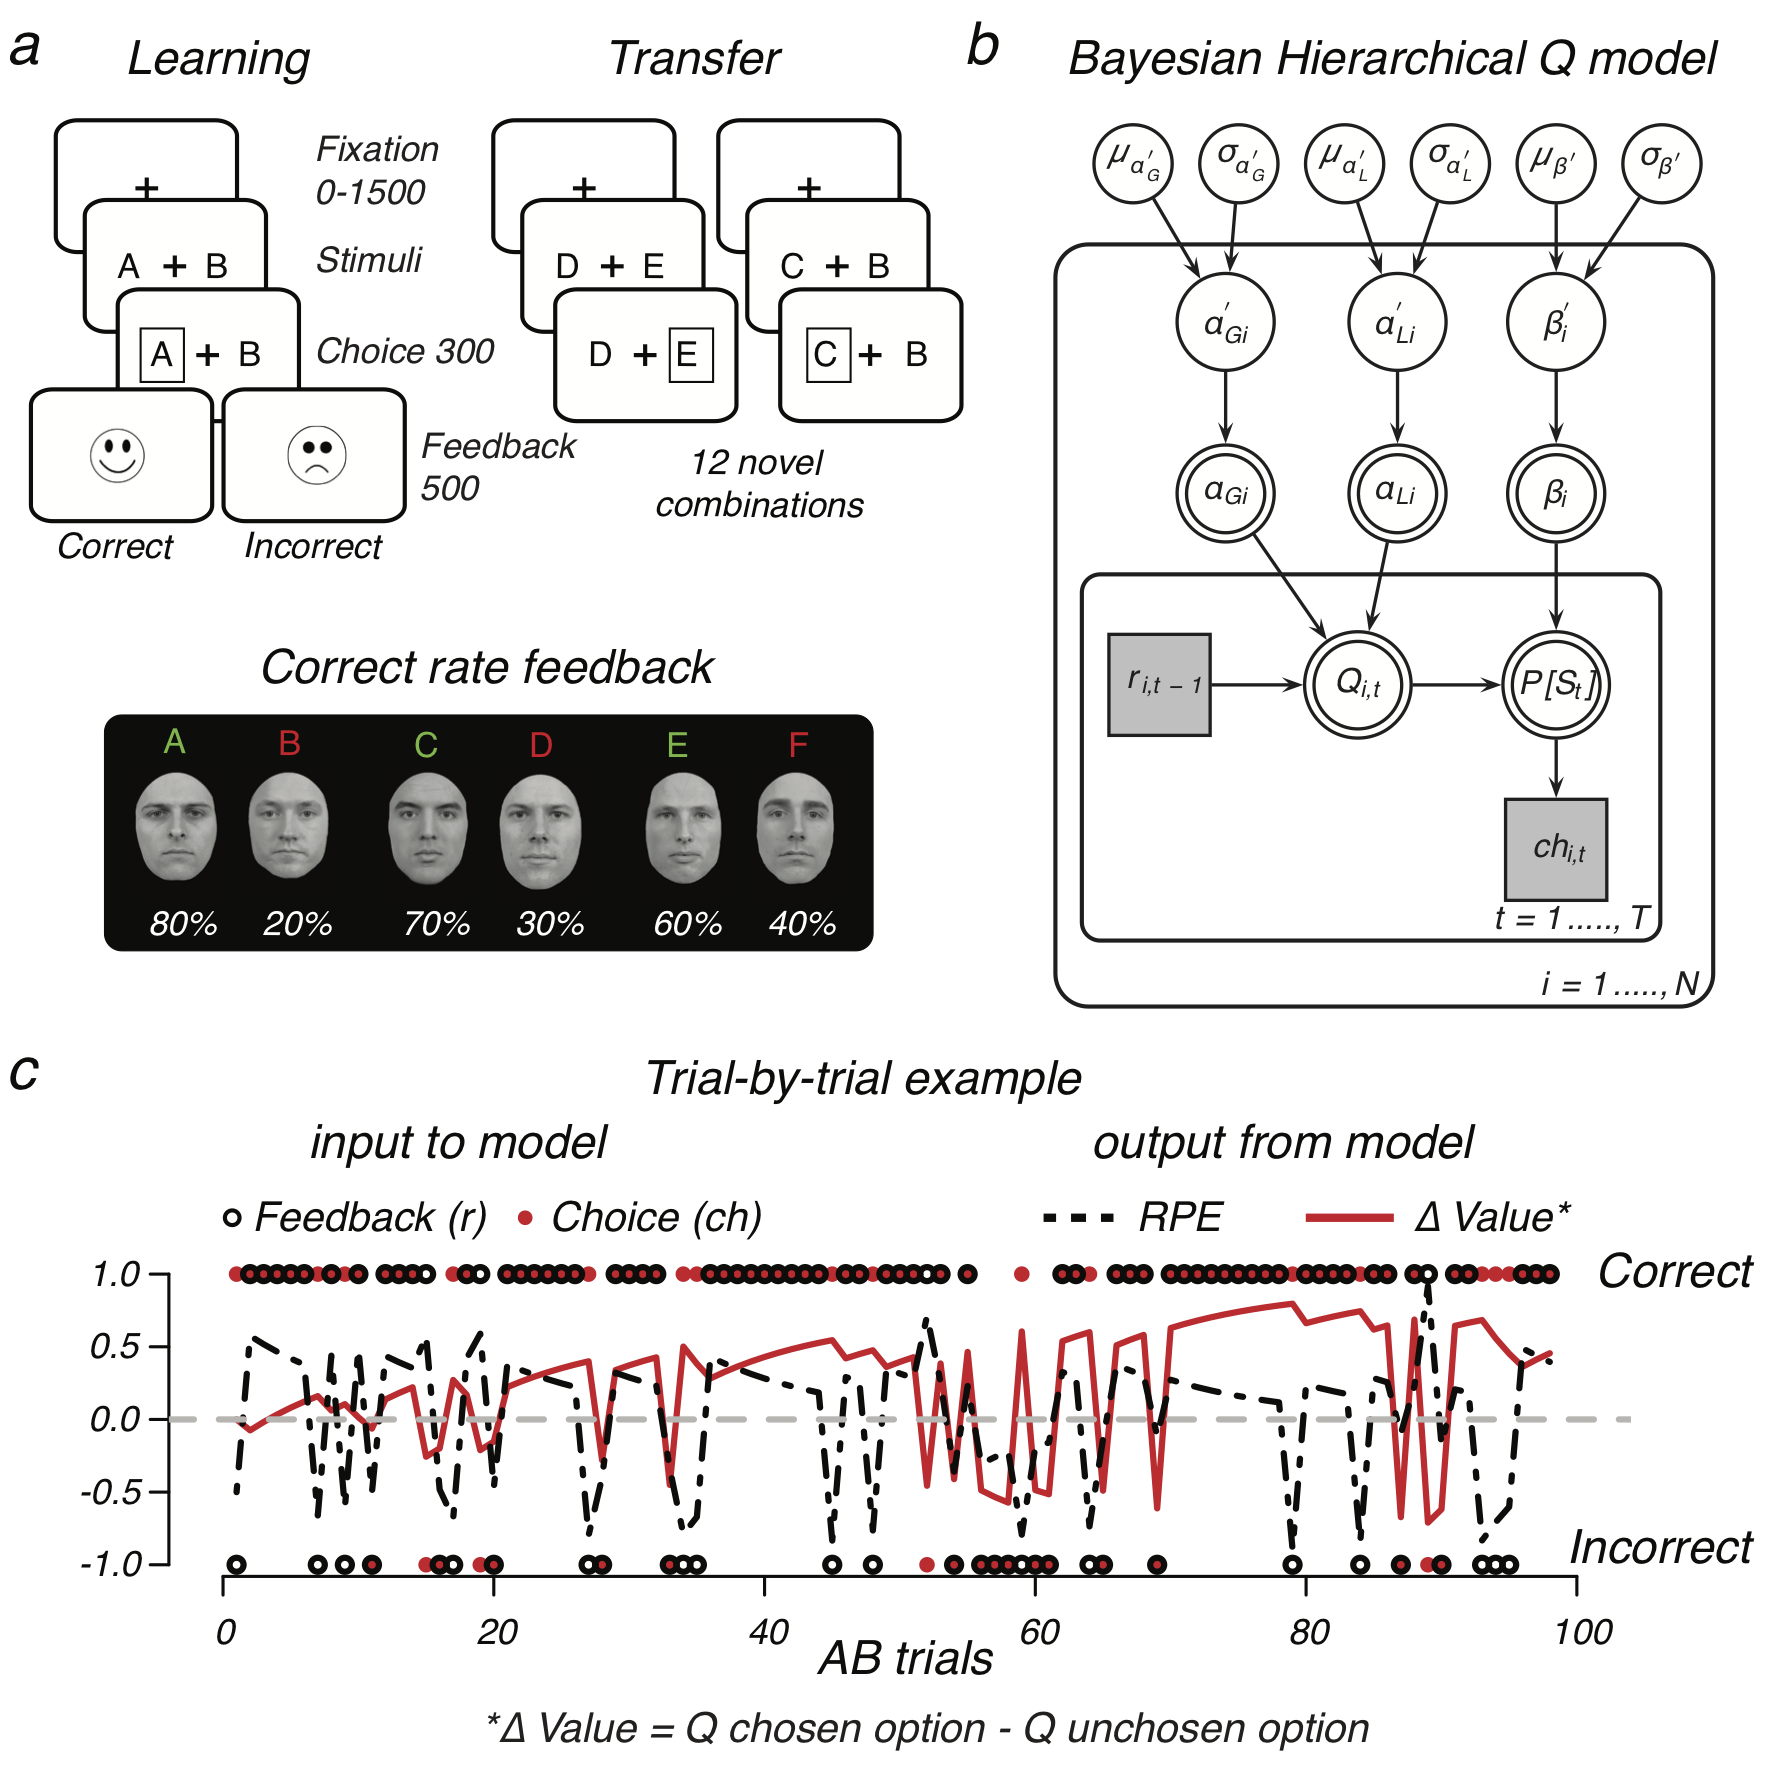
\includegraphics[width=0.8\textwidth,height=\textheight]{_png/Figure1.png}
\caption{\textbf{Design and Model.} (\textbf{a}) Reinforcement learning
task using faces. During learning, two faces were presented on each
trial, and participants learned to select the optimal face identity (A,
C, E) through probabilistic feedback (\% of correct is shown beneath
each stimulus). The learning-phase contained three face pairs (AB, CD,
ED) for which feedback was given. In a follow-up transfer phase these
faces were rearranged into 12 novel combinations to asses learning.
These trials were identical to learning trials, with the exception of
feedback. (\textbf{b}) Graphical \(Q\)-learning model with hierarchical
Bayesian parameter estimation. The model consists of an outer subject
(\(i=1,…..,N\)), and an inner trial plane (\(t=1,…,T\)). Nodes represent
variables of interest. Arrows are used to indicate dependencies between
variables. Double borders indicate deterministic variables. Continuous
variables are denoted with circular nodes, and discrete with square
nodes. Observed variables are shaded in grey (see materials and methods
for details about the fitting procedure). (\textbf{c}) Illustration of
the observed trial-by-trial input (i.e., the choice made, and feedback
received), and output (i.e., \(Q\) for the chosen and unchosen stimulus,
\(\Delta\)Value, and RPE) of the model given the estimated variability
in learning rates from either positive (\(\alpha_{Gi}\)) or negative
(\(\alpha_{Li}\)) feedback, and the tendency to exploit \(\beta\) higher
values \(i\). \label{Figure 1}}
\end{figure}

\hypertarget{materials-and-methods}{%
\section{Materials and Methods}\label{materials-and-methods}}

To understand how value learning relates to the activity pattern in
perceptual regions we reanalyzed the behavioral and fMRI recordings of a
recent study (Jahfari et al. 2018). In this study, BOLD signals were
recorded while participants performed a reinforcement learning task
using male or female faces, and a stop-signal task (which was discussed
in Jahfari et al. (2018)). The fusiform face area (FFA) was localized
using a separate experimental run.

\hypertarget{participants}{%
\subsection{Participants}\label{participants}}

49 young adults (25 male; mean age = 22 years; range 19-29 years)
participated in the study. All participants had normal or
corrected-to-normal vision and provided written consent before the
scanning session, in accordance with the declaration of Helsinki. The
ethics committee of the University of Amsterdam approved the experiment,
and all procedures were in accordance with relevant laws and
institutional guidelines. In total, six participants were excluded from
all analyses due to movement (2), incomplete sessions (3), or
misunderstanding of task instructions (1). In total data from 43
participants was analyzed.

\hypertarget{reinforcement-learning-task}{%
\subsection{Reinforcement learning
task}\label{reinforcement-learning-task}}

Full details of the reinforcement learning task are provided in Jahfari
et al. (2018). In brief, the task consisted of two phases (Figure 1a).
In the first learning phase, three male or female face pairs (AB, CD,
EF) were presented in a random order, and participants learned to select
the most optimal face (A, C, E) in each pair solely through
probabilistic feedback (`correct': happy smiley, `incorrect': sad
smiley). Choosing face-A lead to `correct' on \(80\%\) of the trials,
whereas a choice for face-B only lead to the feedback `correct' for
\(20\%\) of the trials. Other ratios for `correct' were 70:30 (CD) and
60:40 (EF). Participants were not informed about the complementary
relationship in pairs. All trials started with a jitter interval where
only a white fixation cross was presented and had a duration of 0, 500,
1000 or 1500ms to obtain an interpolated temporal resolution of 500ms.
Two faces were then shown left and right of the fixation-cross and
remained on screen up to response, or trial end (4000ms). If a response
was given on time, a white box surrounding the chosen face was then
shown (300ms) and followed (interval 0-450ms) by feedback (500ms).
Omissions were followed by the text `miss' (2000ms). The transfer-phase
contained the three face-pairs from the learning phase, and 12 novel
combinations, in which participants had to select which item they
thought had been more rewarding during learning. Transfer-phase trials
were identical to the learning phase, with the exception that no
feedback was provided. All trials had a fixed duration of 4000ms, where
in addition to the jitter used at the beginning of each trial, null
trials (4000ms) were randomly interspersed across the learning (60
trials; \(20\%\)) and transfer (72 trials; \(20\%\)) phase. Each face
was presented equally often on the left or right side, and choices were
indicated with the right-hand index (left) or middle (right) finger.
Before the MRI session, participants performed a complete learning phase
to familiarize with the task (300 trials with different faces). In the
MRI scanner, participants performed two learning blocks of 150 trials
each (300 trials total; equal numbers of AB, CD and EF), and three
transfer phase blocks of 120 trials each (360 total; 24 presentations of
each pair). All stimuli were presented on a black-projection screen that
was viewed via a mirror-system attached to the MRI head coil.

\hypertarget{reinforcement-learning-model}{%
\subsection{Reinforcement learning
model}\label{reinforcement-learning-model}}

Trial-by-trial updating in value beliefs about the face selected in the
learning phase, and reward prediction errors (signed expectancy
violations) were estimated with a variant of the computational
\(Q\)-learning algorithm (Watkins and Dayan 1992; Frank et al. 2007; Daw
2011) that is frequently used with this reinforcement learning task and
contains two separate learning rate parameters for positive
(\(\alpha_{gain}\)) and negative (\(\alpha_{loss}\)) reward prediction
errors (Frank et al. 2007; Kahnt et al. 2009; Niv et al. 2012; Jahfari
and Theeuwes 2017; Jahfari et al. 2018). \(Q\)-learning assumes
participants to maintain reward expectations for each of the six
(A-to-F) stimuli presented during the learning phase. The expected value
(\(Q\)) for selecting a stimulus \(i\) (could be A-to-F) upon the next
presentation is then updated as follows:

\[
    Q_i(t+1)=  Q_i(t) +
\begin{cases}
    \alpha_{Gain}[r_i(t)-Q_i(t)],& \text{if } r=1\\
    \alpha_{Loss}  [r_i(t)-Q_i(t)],& \text{if } r=0
\end{cases}
\]

Where \(0\leq\) \(\alpha_{gain}\) or \(\alpha_{loss}\) \(\leq 1\)
represent learning rates, \(t\) is trial number, and \(r=1\) (positive
feedback) or \(r=0\) (negative feedback). The probability of selecting
one response over the other (i.e., A over B) is computed as:

\[
    P_A(t)=  \frac{\exp(\beta * Q_t(A))} 
    {\exp(\beta * Q_t(B)) + \exp(\beta * Q_t(A))}
\]

With \(0\leq\) \(\beta\) \(\leq 100\) known as the inverse temperature.

\hypertarget{bayesian-hierarchical-estimation-procedure}{%
\subsection{Bayesian hierarchical estimation
procedure}\label{bayesian-hierarchical-estimation-procedure}}

To fit this \(Q\)-learning algorithm with two learning rate parameters
we used Bayesian hierarchical estimation procedure. The full estimation
procedure is explained in (Jahfari et al. 2018). To summarize, this
implementation assumes that probit-transformed model parameters for each
participant are drawn from a group-level normal distribution
characterized by group level mean and standard deviation parameters:
\(z \sim N(\mu_z, \sigma_z)\). A normal prior was assigned to
group-level means \(\mu_z \sim N(0,1)\), and a uniform prior to the
group-level standard deviations \(\sigma_z \sim U(1,1.5)\). Model fits
were implemented in Stan, where multiple chains were generated to ensure
convergence.

\hypertarget{image-acquisition}{%
\subsection{Image acquisition}\label{image-acquisition}}

The fMRI data for the Reinforcement learning task was acquired in a
single scanning session with two learning and three transfer phase runs
on a 3-T scanner (Philips Achieva TX, Andover, MA) using a 32-channel
head coil. Each scanning run contained 340 functional
\(T2^{*}\)-weighted echo-planar images for the learning phase, and 290
\(T2^{*}\)-weighted echo planar images for the transfer phase (TR = 2000
ms; TE = 27.63 ms; FA = 76.1°; 3 mm slice thickness; 0.3 mm slice
spacing; FOV = 240 × 121.8 × 240; 80 × 80 matrix; 37 slices, ascending
slice order). After a short break of 10 minutes with no scanning, data
collection was continued with a three-dimensional \(T1\) scan for
registration purposes (repetition time {[}TR{]} = 8.5080 ms; echo time
{[}TE{]} = 3.95ms; flip angle {[}FA{]} = 8°; 1 mm slice thickness; 0 mm
slice spacing; field of view {[}FOV{]} = 240 × 220 × 188), the fMRI data
collection using a stop signal task (described in Jahfari et al.
(2018)), and a localizer task with faces, houses, objects, and scrambled
scenes to identify FFA responsive regions on an individual level (317
\(T2^{*}\) weighted echo-planar images; TR = 1500 msec; TE = 27.6 msec;
FA = 70°; 2.5 mm slice thickness; 0.25 mm slice spacing; FOV = 240 ×
79.5 × 240; 96 × 96 matrix; 29 slices, ascending slice order). Here,
participants viewed a series of houses, faces, objects as well as
phase-scrambled scenes. To sustain attention during functional
localization, subjects pressed a button when an image was directly
repeated (\(12.5\%\) likelihood).

\hypertarget{fmri-analysis-learning-phase}{%
\subsection{fMRI analysis learning
phase}\label{fmri-analysis-learning-phase}}

The interplay between learning and perceptual activity was examined by
evaluating how trial-by-trial computations of value-beliefs, and reward
prediction errors relate to BOLD responses in the occipital cortex (OC)
and fusiform face area (FFA). To compare perceptual responses with the
more traditional literature, we first show how value-beliefs and RPEs
relate to the activity pattern of the dorsal (i.e., caudate, or putamen)
or ventral (i.e., accumbens) parts of the striatum. Regions of interest
(ROI) templates were defined using anatomical atlases available in FSL,
or the localizer task for FFA. For this purpose, the localizer scans
were preprocessed using motion correction, slice-time correction, and
pre-whitening (Woolrich et al. 2001). For each subject, a GLM was fitted
with the following EVs: for FFA, faces \(>\) (houses and objects), for

\begin{shaded}PPA\end{shaded}

, houses \(>\) (faces and objects) and for LOC, intact scenes \(>\)
scrambled scenes. Higher-level analysis was performed using FLAME Stage
1 and Stage 2 with automatic outlier detection (Beckmann et al. 2003).
For the whole-brain analysis Z (Gaussianized T/F) statistic images were
thresholded using clusters determined by \(z > 2.3\) and \(p < .05\)
(GRFT) to define a group-level binary FFA region. Templates used for the
caudate {[}center of gravity (cog): (-) 13, 10, 10{]}, putamen {[}cog:
(-) 25, 1, 1{]}, and nucleus accumbens {[}cog: (-)19, 12, -7{]} were
based on binary masks. Because participants were asked to differentiate
faces, for each participant, we multiplied the binary templates of OC
(V1) {[}cog: 1, -83, 5{]}, FFA {[}cog: 23, -48, -18{]} with the
individual t-stats from the localizer task contrast faces \(>\) (houses
and objects). All anatomical masks, and the localizer group-level FFA
mask can be downloaded from github (see acknowledgements).

\hypertarget{deconvolution-analysis-learning-phase}{%
\subsection{Deconvolution analysis learning
phase}\label{deconvolution-analysis-learning-phase}}

To more precisely examine the time course of activation in the striatal
and perceptual regions, we performed finite impulse response estimation
(FIR) on the BOLD signals. After motion correction, temporal filtering
(3rd order savitzky-golay filter with window of 120 s) and percent
signal change conversion, data from each region was averaged across
voxels while weighting voxels according to ROI probability masks, and
upsampled from 0.5 to 3 Hz. This allows the FIR fitting procedure to
capitalize on the random timings (relative to TR onset) of the stimulus
presentation and feedback events in the experiment. Separate response
time courses were simultaneously estimated triggered on two separate
events: stimulus onset, feedback onset. FIR time courses for all trial
types were estimated simultaneously using a penalized (ridge)
least-squares fit, as implemented in the FIRDeconvolution package
(Knapen and Gee 2016), and the appropriate penalization parameter was
estimated using cross-validation. For stimulus onset events (i.e., onset
presentation of face pairs) response time courses were fit separately
for the AB, CD and EF pairs, while also estimating the time courses of
signal covariation with chosen and unchosen value for these pairs. For
these events, our analysis corrected for the duration of the decision
process. For the feedback events, the co-variation response time course
with signed and unsigned prediction errors were estimated. These signal
response time courses were analysed using across-subjects GLMs at each
time-point using the statsmodels package (Seabold and Perktold 2010).
The \(\alpha\) value for the contributions of \(Q\) or RPE was set to
\(0.0125\) (i.e.~a Bonferroni corrected value of \(0.05\) given the
interval of interest between 0 and 8 s).

\hypertarget{random-forest-classification}{%
\subsection{Random Forest
classification}\label{random-forest-classification}}

To specify the relevance of perceptual regions in the resolve of future
value-driven choices a random forest (RF) classifier was used (Breiman
2001, 2004). The RF classifier relies on an ensemble of decision trees
as base learners, where the final prediction (e.g., for a given trial is
the choice going to be correct/optimal? or incorrect/suboptimal? given
past learning) is obtained by a majority vote that combines the
prediction of all decision trees. To achieve controlled variation, each
decision tree is trained on a random subset of the variables
(i.e.~regions of interest chosen), and a bootstrapped sample of data
points (i.e.~trials). In the construction of each tree about 1/3 of all
trials is left out - termed as the out-of-bag sample -- and later used
to see how well each tree preforms on unseen data. The generalized error
for predictions is calculated by aggregating the prediction for every
out-of-bag sample across all trees. An important feature of the RF
classification method is the ease to measure the relative importance of
each variable (i.e., region), in the overall predictive performance.
That is, it allows for the ranking of all regions evaluated in the
prediction of future value-based decisions.

\hypertarget{roi-selection-and-random-forest-procedure}{%
\subsection{ROI selection and Random Forest
procedure}\label{roi-selection-and-random-forest-procedure}}

This study used the `Breiman and Cutler's Random Forests for
Classification and Regression' package in R, termed randomForest. RF
evaluations relied on the fMRI data recorded during the transfer phase,
in a set of 9 regions of interest (ROIs). These ROIs included all
templates from the learning phase (i.e., caudate, putamen, accumbens,
OC, and FFA), as well as, the ventromedial prefrontal cortex (vmPFC),
dorsolateral prefrontal cortex (DLPFC), pre-supplementary motor area
(preSMA), and the primary motor cortex (M1). The selection of these
additional anatomical templates was inspired by our previous analysis of
this data with those templates focusing on networks (Pircalabelu et al.
2015; Schmittmann et al. 2015; Jahfari et al. 2018). From each ROI a
single parameter estimate (averaged normalized \(\beta\) estimate across
voxels in each ROI) was obtained per trial, per subject. All,
pre-processing steps to obtain single-trial images are described in
Jahfari et al. (2018). Single-trial activity estimates were used as
input variables in RF to predict choice outcomes (optimal/sub-optimal)
in the transfer phase. Here, participants choose the best/optimal option
based on values learned during the learning phase. We defined optimal
choices as correct (i.e, when participants choose the option with the
higher value), and sub-optimal choices as incorrect. Misses were
excluded from RF evaluations.

By design, the transfer-phase contained 360 trials including 15
different pairs (12 novel), where each pair was presented 24 times with
the higher value presented left in 12 of the 24 presentations, and on
the right for the other half. With so many subtle value differences
across the options presented and only one BOLD estimate per trial/region
the prediction of future choices is under powered (Figure 2a).
Therefore, assuming that all participants come from the same population,
a fixed effects approach was taken for evaluations with RF. Here, the
trial\(*\)region activity matrices for all participants were combined
into one big data matrix (Figure 2b) and subsequently shuffled across
the rows, so that both participants and trials were re-arranged in a
random order across rows. Besides the single trial BOLD estimates from
the 9 ROI's, this shuffled matrix contained two additional columns,
which specified subject\_id (to which subject does each trial belong),
and Trial Sign -- i.e., is the choice between the two faces about two
positive (+/+; AC, AE, CE), negative (-/-; BD, BF, DF), or a
positive-negative (+/-; e.g.~AD, CF etc. ) associations given the task
manipulation during learning. Subject\_id was included to control for
different BOLD fluctuations across participants, whereas Trial Sign was
added because both BOLD and choice patterns differ across these options
(please see Jahfari et al. (2018)). The shuffled fixed effect matrix was
divided into a separate training (2/3 of whole matrix), and validation
(1/3) set, to be used for RF evaluations (Figure 2c). Learning was based
on the training set, using 2000 trees with the number of variables
(regions) used by each tree optimized with the tuneRF function in R, and
accordingly set to 5. For the construction of each tree about 1/3 of all
trials is left out - termed as the out-of-bag sample -- and later used
to see how well each tree preforms on unseen data. The generalized error
for predictions is calculated by aggregating the prediction for every
out-of-bag sample across all trees. Besides this out-of-bag
approximation we evaluated the predictive accuracy of the whole RF on
the separate unseen validation-set. The single trial data used as input,
the RF evaluation codes, and ROI templates can all be downloaded from
the github link provided in acknowledgements.

\begin{figure}
\centering
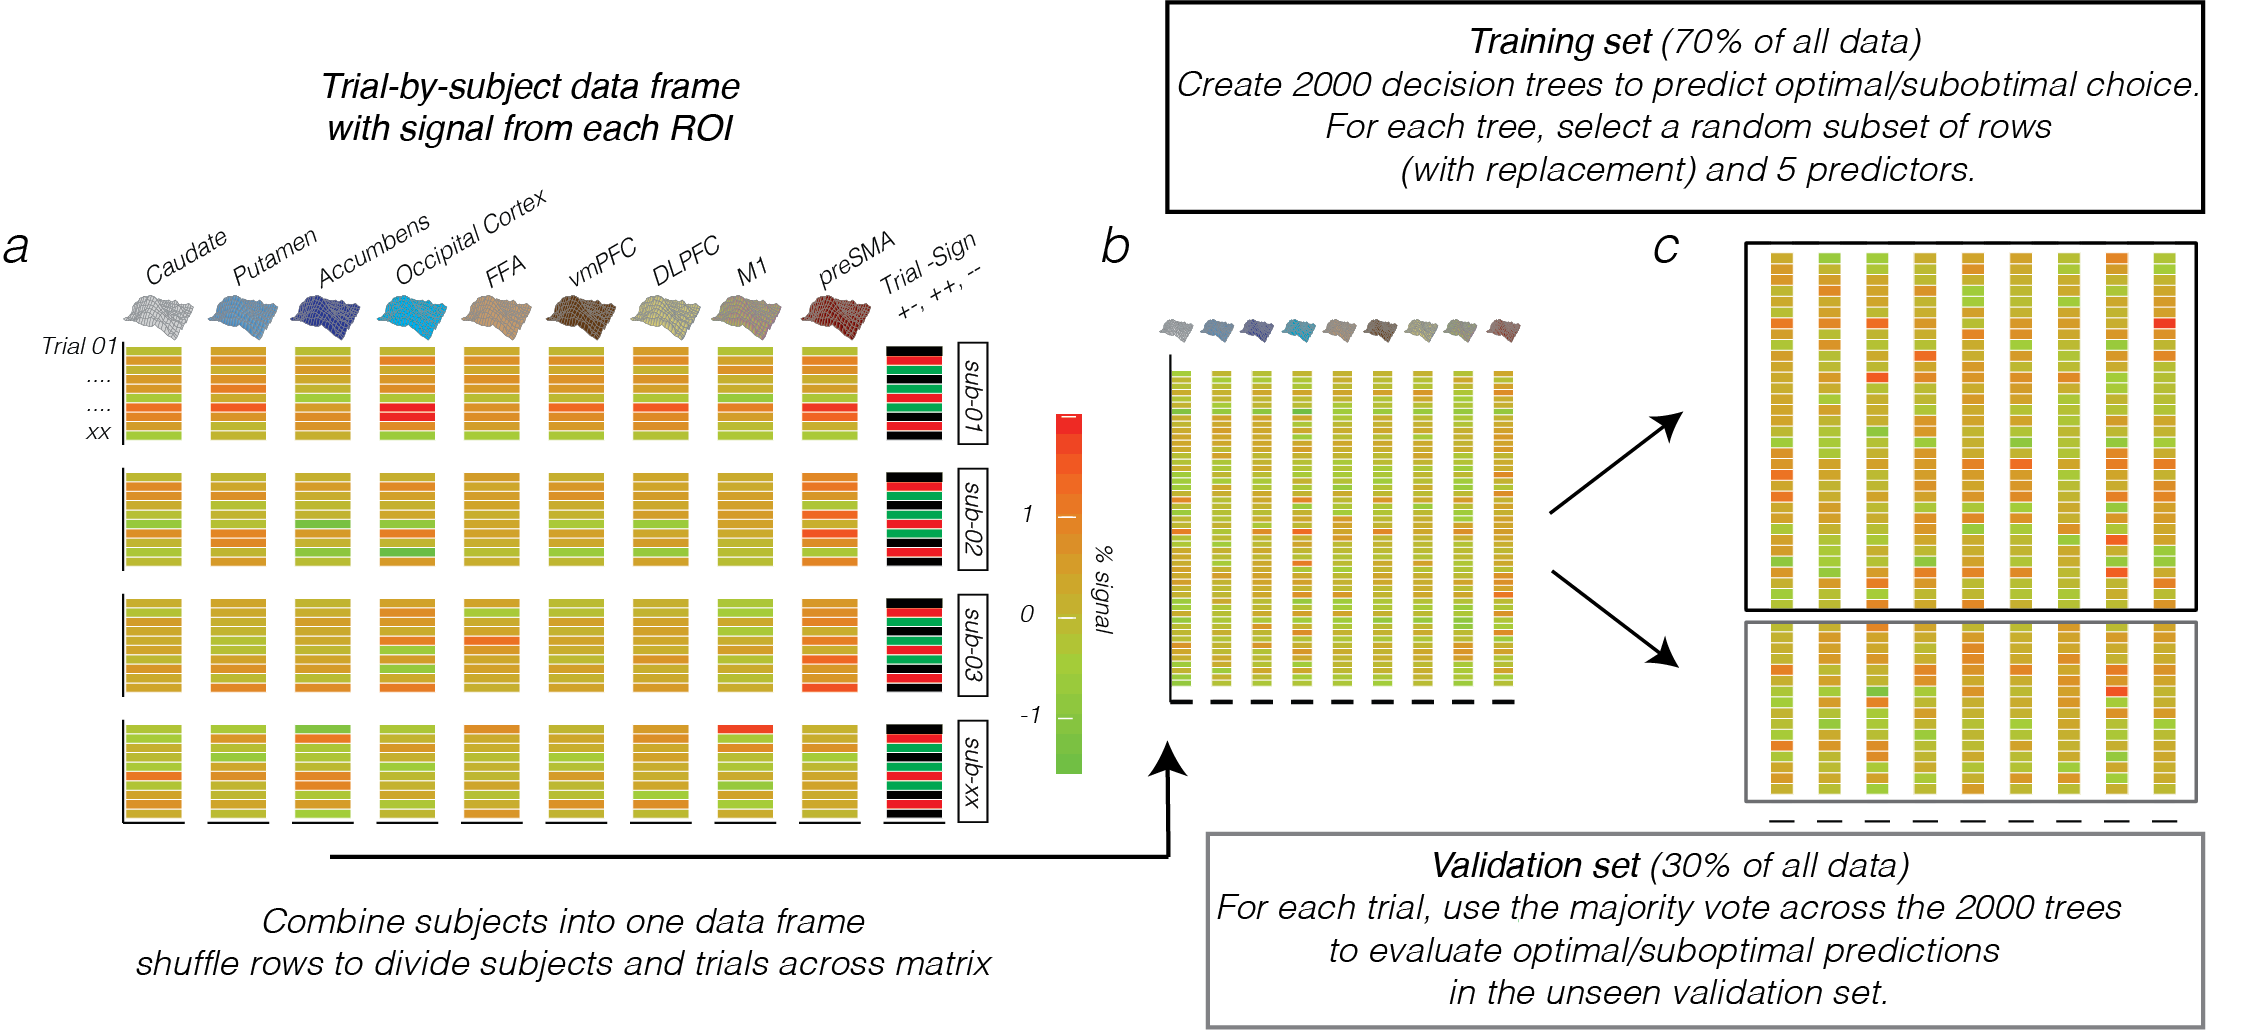
\includegraphics{_png/Figure5.png}
\caption{\textbf{Random Forest input and data-structure.} (\textbf{a})
Trial-by-subject data matrix with the \(\%\) signal change drawn for
each choice trial in the transfer-phase (rows) from \(9\) a-priori
defined regions of interest (columns). In addition to the ROI data, the
matrix contained a column with the identity of participants (sub-01,
etc) and Trial Sign, which specified a choice between two positives
(+/+; AC, AE, CE), negatives (-/-, BD, BF, DF), or between a negative
and positive option (+/-, e.g., AD, CF, etc) given the feedback scheme
in the learning-phase. (\textbf{b}) The individual subject data frames
were then combined into one matrix, in which the rows were subsequently
shuffled to randomly distribute trials and subjects across the rows.
(\textbf{c}) This matrix was then divided into a training set (2/3 of
the data) for the creation of 2000 decision trees of which the majority
vote on each trial is then used to evaluate the predictive accuracy of
optimal/suboptimal choices in a separate validation set (1/3 of the
data). \label{Figure 2}}
\end{figure}

\hypertarget{results}{%
\section{Results}\label{results}}

\hypertarget{model-and-behavior}{%
\subsection{Model and Behavior}\label{model-and-behavior}}

As shown in Figure 1a, in the reinforcement learning task participants
learned to select among choices with different probabilities of
reinforcement (i.e., AB 80:20, CD 70:30, and EF 60:40). A subsequent
transfer phase, where feedback was omitted, required participants to
select the optimal option among novel pair combinations of the faces
that were used during the learning phase (Figure 1a). In the learning
phase, subjects reliably learned to choose the most optimal face option
in all pairs. For each pair the probability of choosing the better
option was above chance (\(p\)'s \(< .001\)), and the effect of learning
decreased from AB (80:20) and CD (70:30) to the most uncertain EF
(60:40) pair (\(F(2, 84) = 13.74, p < .0001\)). At the end of learning,
value beliefs differentiating the optimal (A, C, E) from the sub-optimal
(B, D, F) action were very distinct for the AB and CD face pairs but
decreased with uncertainty (\(F(2,84)=39.70, p<0.0001\), Figure 3a).
Value beliefs were estimated using the individual subject parameters of
the \(Q\)-learning model that best captured the observed data (Figure
3b-e; reproduced from Jahfari et al. (2018) to show performance).

\begin{figure}
\centering
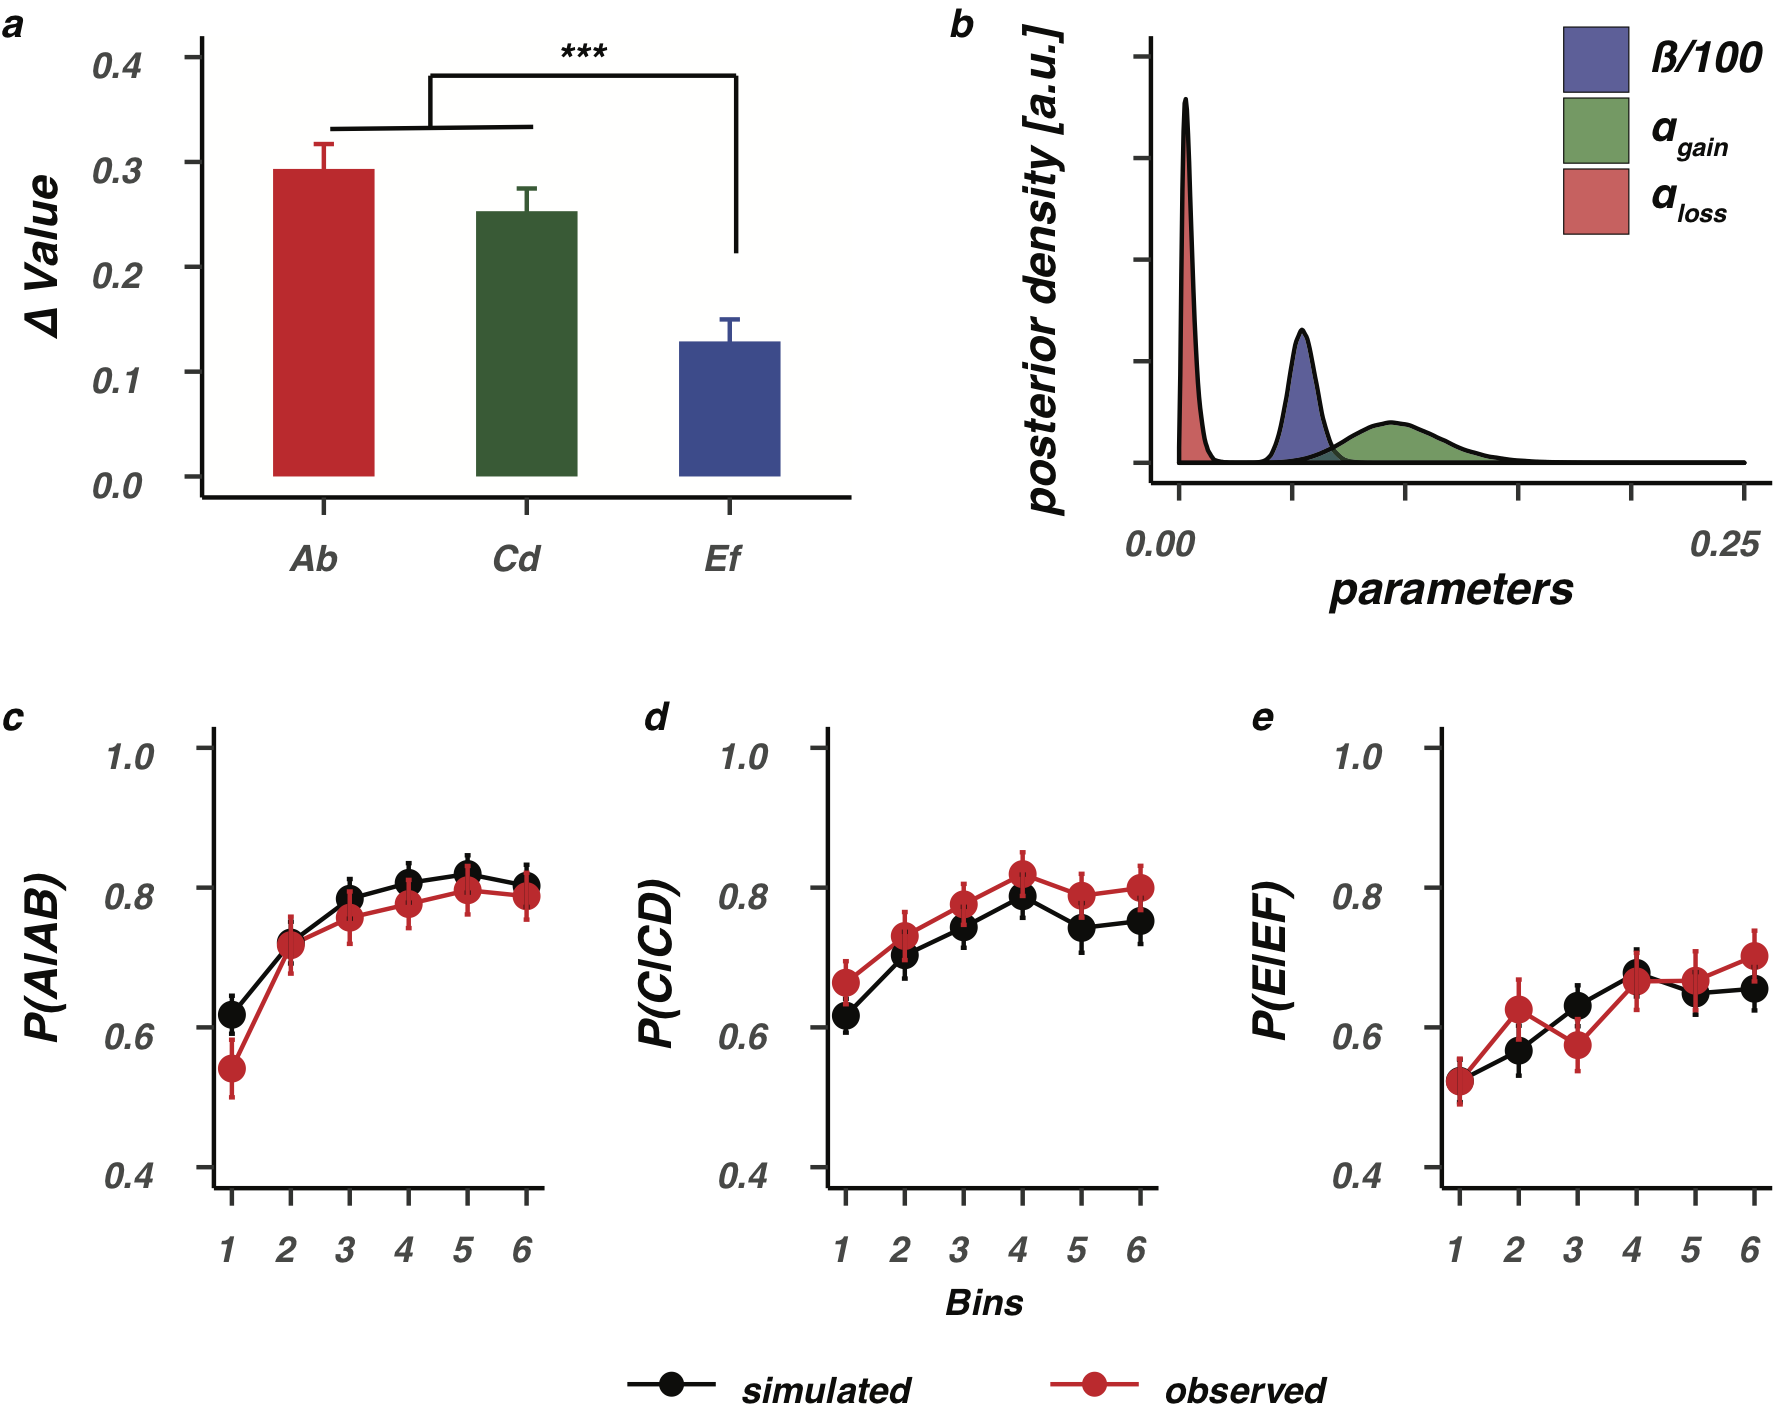
\includegraphics[width=0.6\textwidth,height=\textheight]{_png/Figure2.png}
\caption{\textbf{Value differentiation and model performance.}
(\textbf{a}) Value differentiation (\(\Delta\)Value) for the selection
of the optimal (A,C,E) stimuli over the suboptimal (B,D,F) stimuli
decreased as a function of feedback reliability, and was smallest for
the most uncertain EF stimuli. \(*** = p<0.0001\), Bonferroni corrected.
(\textbf{b}) Group-level posteriors for all \(Q\)-learning parameters.
The bottom row shows model performance, where data was simulated with
the estimated individual subject parameters and evaluated against the
observed data for the AB (\textbf{c}), CD (\textbf{d}), or EF
(\textbf{e}) pairs. Bins contain \(+/-\) 16 trials. Error bars represent
standard error of the mean (SEM). \label{Figure 3}}
\end{figure}

\hypertarget{bold-is-modulated-by-reliable-value-differences-between-faces-in-striatal-and-visual-regions}{%
\subsection{BOLD is modulated by reliable value differences between
faces in striatal and visual
regions}\label{bold-is-modulated-by-reliable-value-differences-between-faces-in-striatal-and-visual-regions}}

For each pair of faces presented during the learning phase (AB, CD, EF)
we asked how the BOLD signal time-course in striatal and visual regions
relates to trial-by-trial value beliefs about the two faces presented as
a choice. First, as a reference, we focused on the activity pattern of
three striatal regions. Results showed BOLD responses in dorsal
(caudate, putamen) but not ventral (accumbens) striatum to be
differentially modulated by the estimated value beliefs of the chosen
face (\(Q_{chosen}\)), in comparison to value beliefs about the face
that was not chosen (\(Q_{unchosen}\)). Thus, BOLD responses in the
dorsal striatum were modulated more strongly by value beliefs about the
chosen stimulus (\(Q_{chosen}\); Figure 4a bottom row). Critically, this
differential modulation was only observed with the presentation of AB
faces where value differences were most distinct because of the reliable
feedback scheme. Next, we evaluated the relationship between value and
BOLD in the FFA, and OC. Again, only with the presentation of the AB
face option, trial-by-trial BOLD fluctuations were differentially
modulated by values of the chosen versus not chosen face option (Figure
4b bottom row). These evaluations highlight how the BOLD response in
striatal and perceptual regions is especially sensitive to values of the
(to-be) chosen stimulus when belief representations are stable and
distinct.

\begin{figure}
\centering
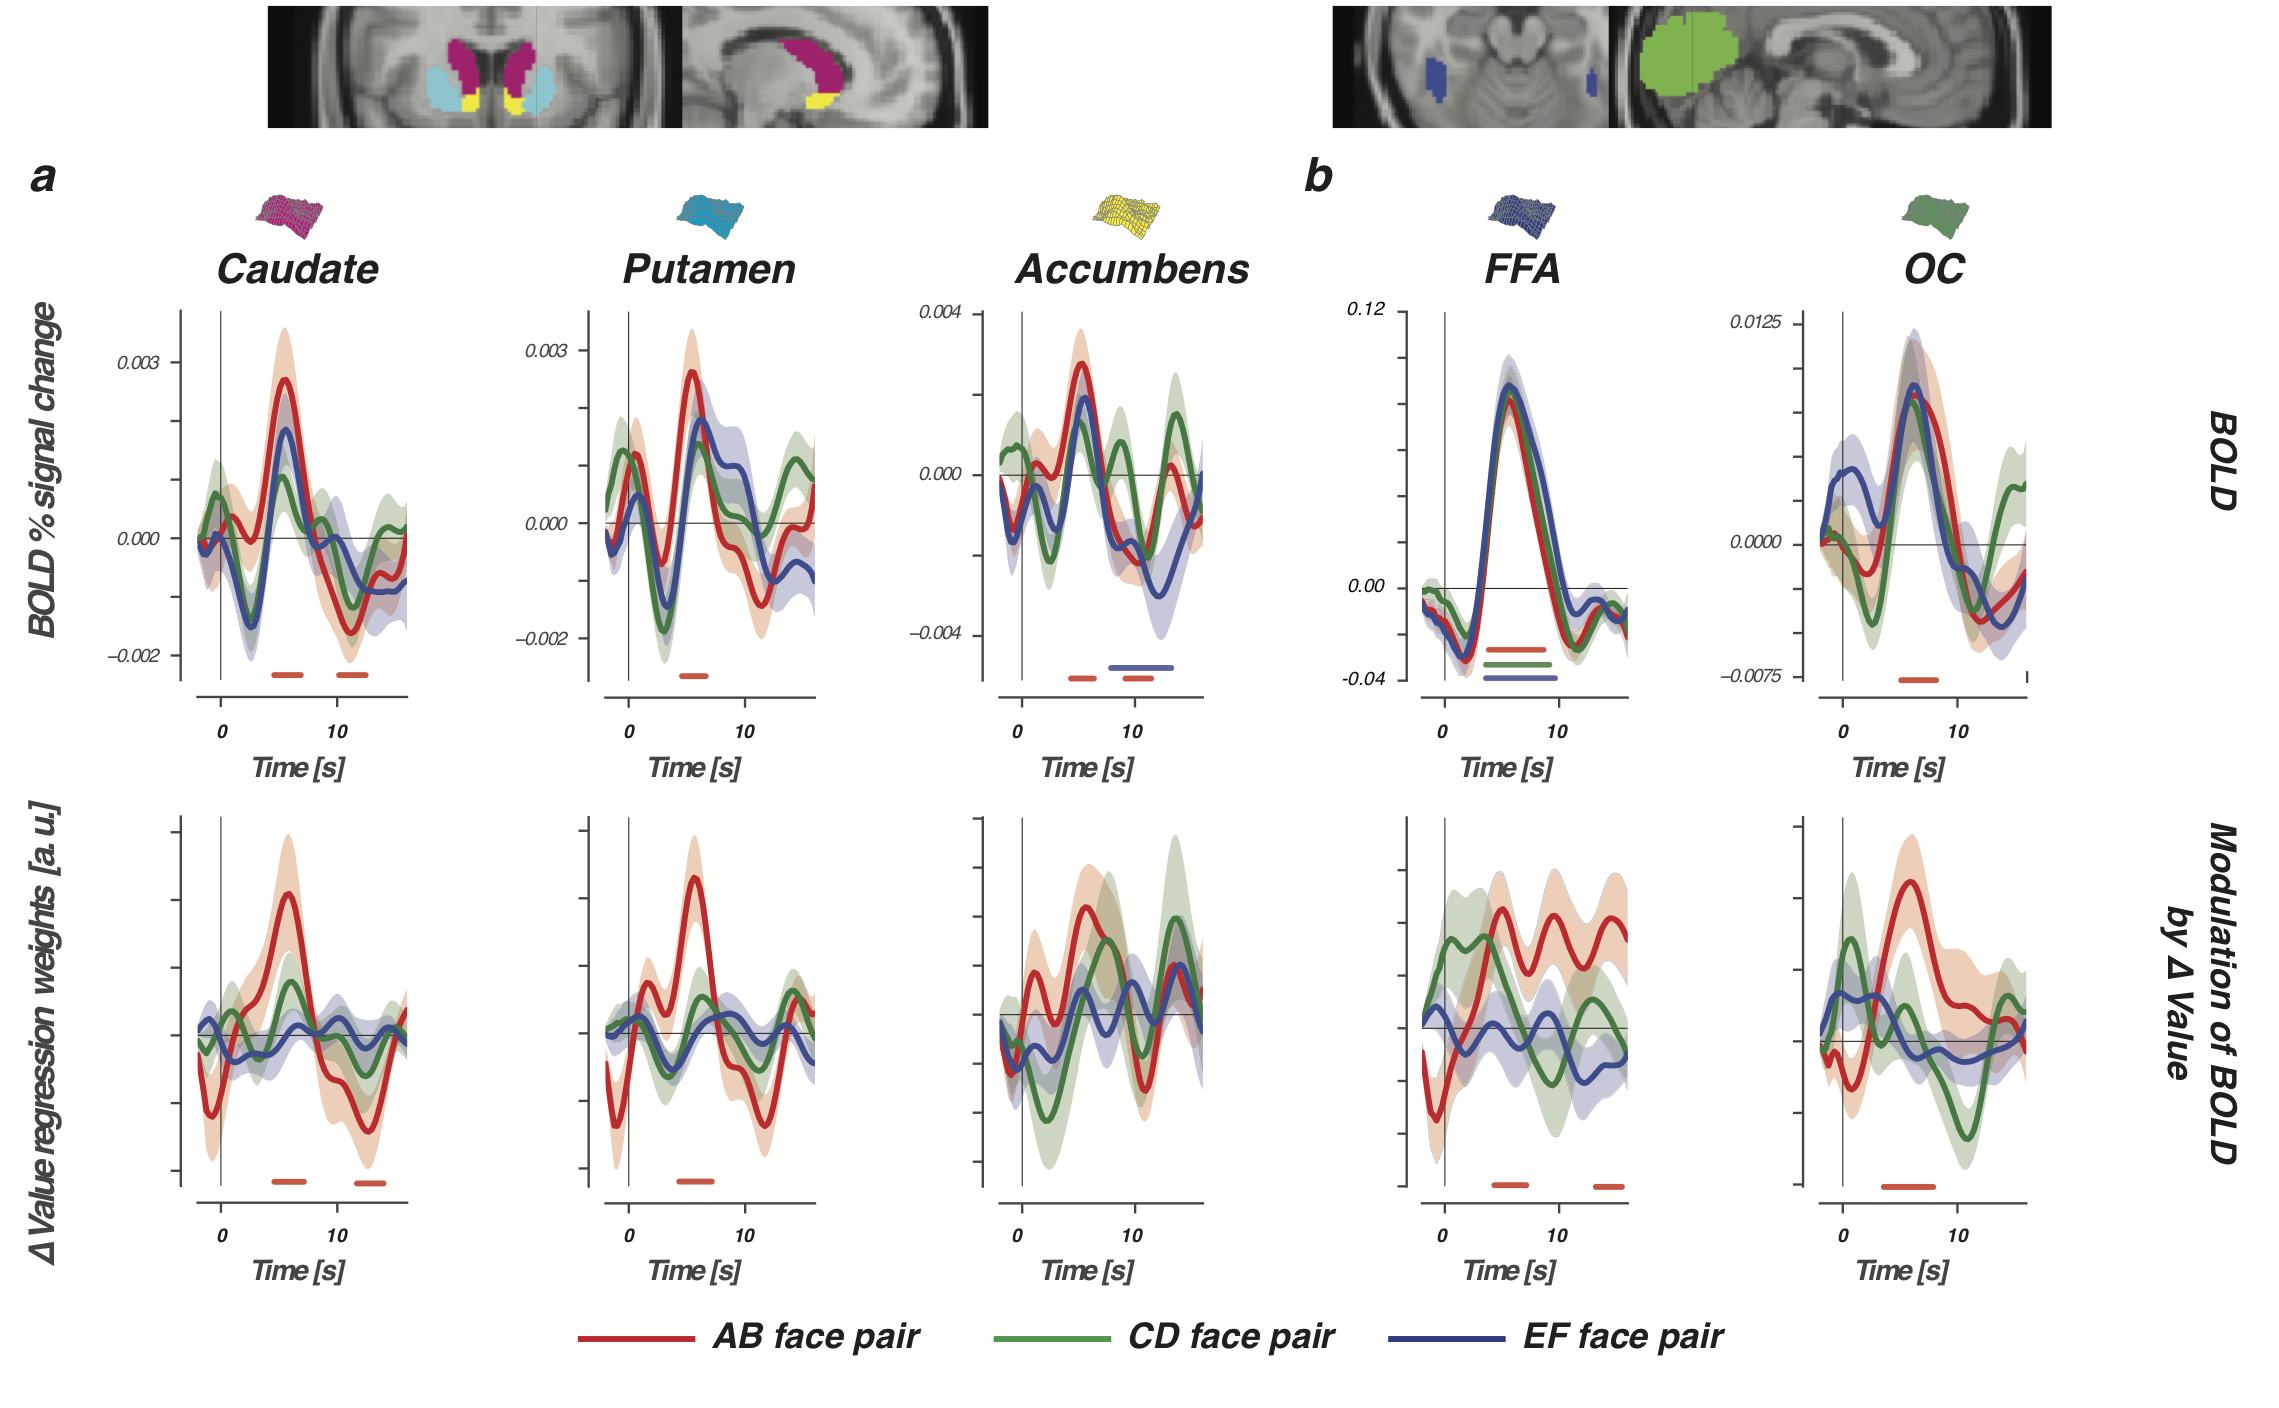
\includegraphics{_png/Figure3.png}
\caption{\textbf{BOLD and the modulation of \(\Delta\)Value in the
learning phase.} Top row shows the BOLD signal time course, time-locked
to presentations of AB (80:20, red lines), CD (70:30, green lines), and
EF (60:40, blue lines) face pairs, for three striatal regions
(\textbf{a}) and two perceptual regions (\textbf{b}). Bottom row
displays differential modulation by value (\(\Delta\)Value = modulation
\(Q_{chosen}\) -- modulation \(Q_{unchosen}\)). Horizontal lines show
the interval in which modulation was significantly stronger for
\(Q_{chosen}\). With the presentation of AB faces, BOLD responses in the
dorsal striatum (caudate and putamen) and visual regions (FFA and OC)
were modulated more by values of the chosen stimulus when compared to
values of the unchosen stimulus. Differential AB value modulation was
not significant in the ventral striatum (i.e., accumbens). Nor did we
observe any differential value modulations with the presentation of the
more uncertain CD and EF pairs. Confidence intervals were estimated
using bootstrap analysis across participants (\(n=1000\)), where the
shaded region represents the standard error of the mean across
participants (bootstrapped \(68\%\) confidence interval).
\label{Figure 4}}
\end{figure}

\hypertarget{reward-prediction-errors-in-striatal-and-visual-regions}{%
\subsection{Reward prediction errors in striatal and visual
regions}\label{reward-prediction-errors-in-striatal-and-visual-regions}}

Our findings so far described relationships between BOLD and value
time-locked to the moment of stimulus presentation -- i.e., when a
choice is requested. Learning occurs when an outcome is different from
what was expected. We therefore next focused on modulations of the BOLD
response when participants received feedback. Learning modulations were
explored by asking how trial-by-trial BOLD responses in perceptual and
striatal regions relate to either signed (outcome was better or worse
than expected) or unsigned (magnitude of expected violation) reward
prediction errors (Fouragnan et al. 2018). Consistent with the
literature, BOLD responses in all striatal regions were modulated by
signed RPEs, with larger responses after positive RPEs or smaller
responses after negative RPEs (Figure 5a bottom row). Activity in the
accumbens (ventral striatum) was additionally tied to unsigned RPEs in
the tail of the BOLD time-course, with larger violations (either
positive or negative) tied to smaller dips. Consistently, estimated BOLD
responses in both visual regions were modulated by the signed RPE, and
once more mirrored the striatal modulations with stronger positive RPEs
eliciting stronger BOLD responses (Figure 5b bottom row). FFA BOLD
responses were additionally modulated by unsigned RPEs. However, in
contrast to the relationship found between unsigned RPEs and the
accumbens, the FFA modulation was positive and co-occurred with the
modulation of the signed RPE. That is, bigger violations and more
positive outcomes each elicited a stronger response in the FFA.

\begin{figure}
\centering
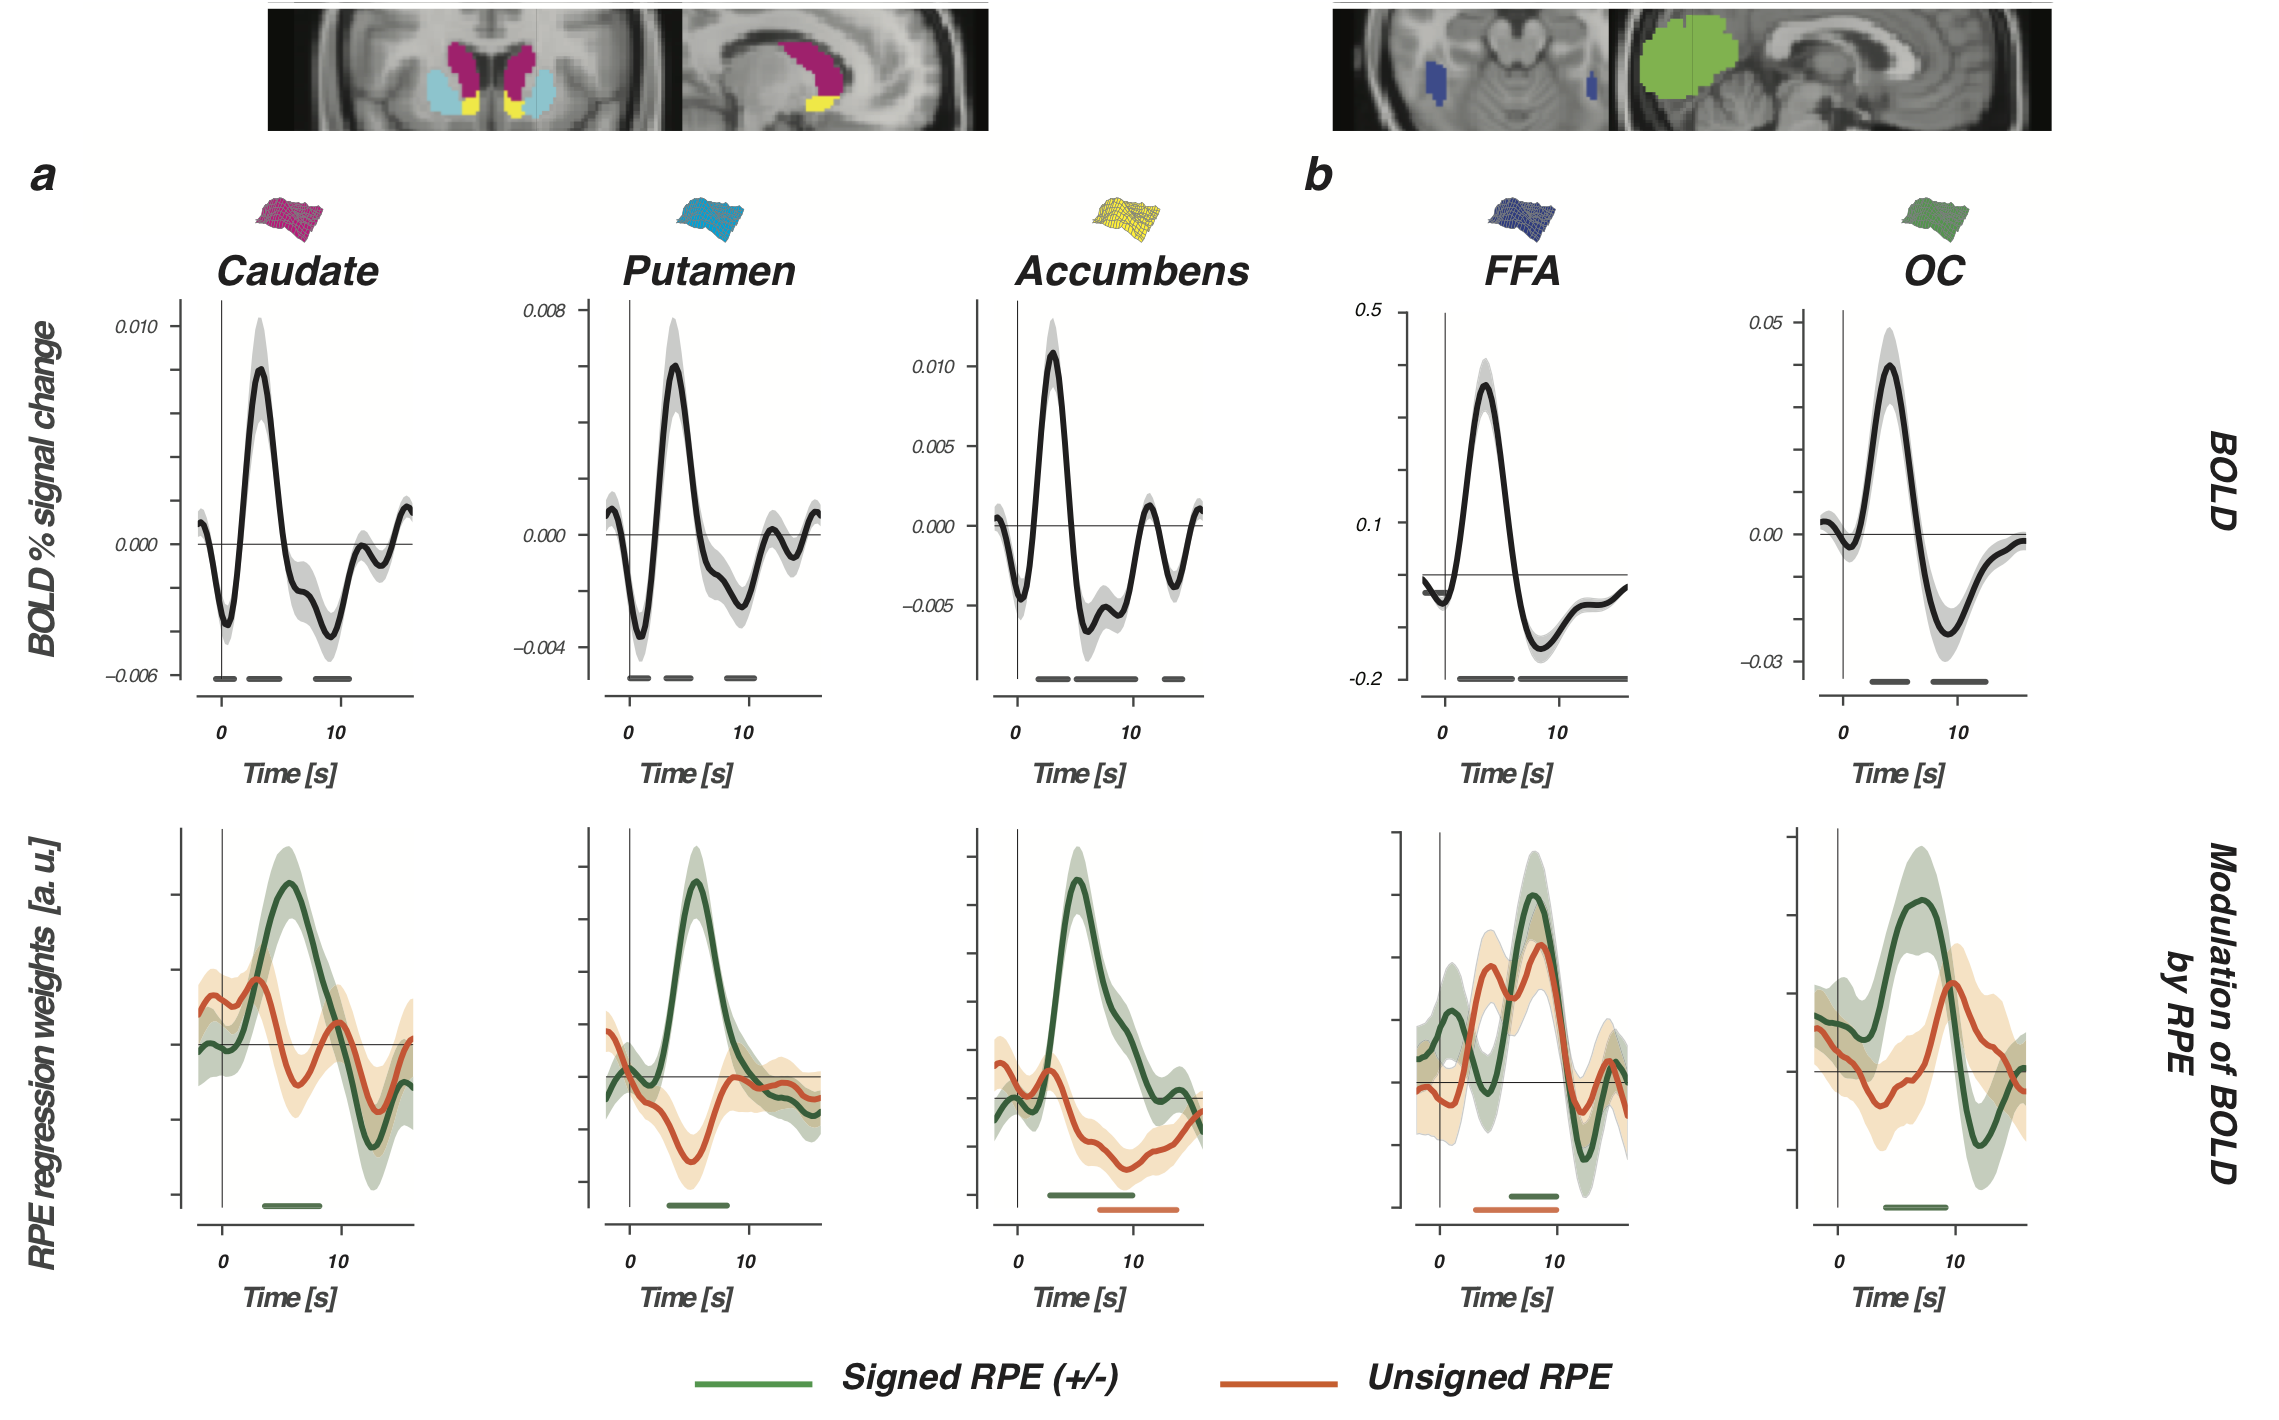
\includegraphics{_png/Figure4.png}
\caption{\textbf{Reward prediction errors modulate BOLD in striatal and
visual regions.} The top row shows the FIR-estimated BOLD signal
time-course, which was time-locked to the presentation of choice
feedback and evaluated for three striatal regions (\textbf{a}) and two
perceptual regions (\textbf{b}). Bottom row displays modulations of the
estimated BOLD time-course by singed (green lines), or unsigned (orange
lines) RPEs. The horizontal lines represent the interval in which signed
or unsigned RPEs contributed significantly to the modulation of BOLD in
the multiple regression. Note that both variables were always evaluated
simultaneously in one GLM. \label{Figure 5}}
\end{figure}

\hypertarget{can-past-learning-in-visual-regions-support-the-prediction-of-future-value-based-decisions}{%
\subsection{Can past learning in visual regions support the prediction
of future value-based
decisions?}\label{can-past-learning-in-visual-regions-support-the-prediction-of-future-value-based-decisions}}

Stable value representations and reward prediction errors both modulated
the activity of visual and striatal regions. These modulations in the
striatum are described to bias future actions towards the most favored
option (the dorsal striatum), or to predict future reward outcomes (the
ventral striatum). To better understand the value and RPE modulations
observed in visual regions, we next assessed the importance of these
visual regions alongside the striatum in the correct classification
(decoding) of future value-driven choice outcomes. Here, activity of
prefrontal regions was added to the importance evaluation based on our
previous work with this data in the transfer phase (Jahfari et al. 2018)
(please see supplementary Figures \(1\&2\) for the evaluation of these
regions during learning).

In the transfer phase, participants had to make a value-driven choice
based on what was learned before, i.e., during the learning phase. To
specify the relevance of visual regions in the resolve of value-driven
choice outcomes, in the transfer phase, a random forest (RF) classifier
was used (Breiman 2001, 2004) (Please see Figure 2a-c for the
procedure). The RF classifier relies on an ensemble of decision trees as
base learners, where the prediction of each trial outcome is obtained by
a majority vote that combines the prediction of all decision trees
(Figure 6a). To achieve controlled variation, each decision tree is
trained on a random subset of the variables (i.e.~subset of columns
shown in Figure 6a), and a bootstrapped sample of data points
(i.e.~trials). Importantly, we ensured that the forest was not simply
learning the proportion of optimal choices in the transfer phase by
training all models on balanced draws from the training set with equal
numbers of optimal and sub-optimal choices.

Evaluation of all participants resulted in a classification accuracy of
\(65\%\) (\(AUC=0.75\)) using the trial-by-trial BOLD estimates from the
ROIs and increased to \(69\%\) with the evaluation of the good learners
(\(AUC=0.76\); \(N=34\), criteria: accuracy \textgreater{} \(60\%\)
across all three learning pairs). Hence, in \(65\) (all participants) or
\(69\) (good learners) out of \(100\) trials the forest correctly
classified whether participants would pick the option with the highest
value (optimal choice) or not (sub-optimal choice) in the validation
set. RF predictions were substantially lower when labels of the
validation set were randomly shuffled (accuracy: all
participants\(=52\%\); good learners\(=56\%\)).

The improvement of accuracy with the evaluation of only the good
learners is remarkable because the classifier was given less data to
learn the correct labelling (fewer subjects/trials) and implied that the
2000 decision trees were picking up information related to past
learning. Further support for this important observation was found by
asking how the uncertainty of each prediction (defined as the proportion
of agreement in the predicted outcome among the 2000 trees for each
trial) relates to the difference in value beliefs (\(\Delta\)Value)
about the two options presented on each trial (computed using the end
\(Q_{beliefs}\) of participants at the end of learning about face
A-to-F). As plotted in Figure 6c, the uncertainty in predicting that a
trial choice outcome is optimal -- defined as the proportion of
disagreement among the 2000 decision trees - decreased with larger
belief differences in the assigned values (please see supplementary
Figure 3 for the evaluation of all participants).

Besides providing insights into how BOLD responses in the transfer-phase
contribute to predict value-driven choice outcomes (i.e., whether
participants would choose the option with the highest value given past
learning) the RF algorithm additionally outputs a hierarchy, thereby
ranking the contribution of each region in the achieved classification
accuracy. Figure 6d shows the ranking of all ROIs for good learners
where the model had the highest predictive accuracy. First, regions in
the dorsal striatum were most important, which aligned well with both
the literature and the BOLD modulations we found by \(\Delta\)Value and
RPE during the learning phase. These regions were next followed by the
preSMA. Evaluation of this region during the learning phase showed no
modulations by \(\Delta\)Value or RPE on BOLD ( supplementary Figure
\(1\&2\)). Nevertheless, this region is typically associated with choice
difficulty/conflict and might be essential in the resolve of a choice
when value differences are small. Remarkably, the third region in this
hierarchy was the FFA. In a task where participants pick the most valued
face based on past learning, this ranking of the FFA just above the
vmPFC and accumbens (ventral striatum) implies that the \(\Delta\)Value
and RPE modulations of BOLD observed during learning could function to
strengthen the recognition of valuable features. Note, however, that
with the evaluation of all participants -- including some who were less
good in learning -- the ranking of both the FFA and vmPFC was much lower
(please see supplementary Figure 3b), which might be caused by more
noise across the group in learning. We will return to this point in the
discussion.

\begin{figure}
\centering
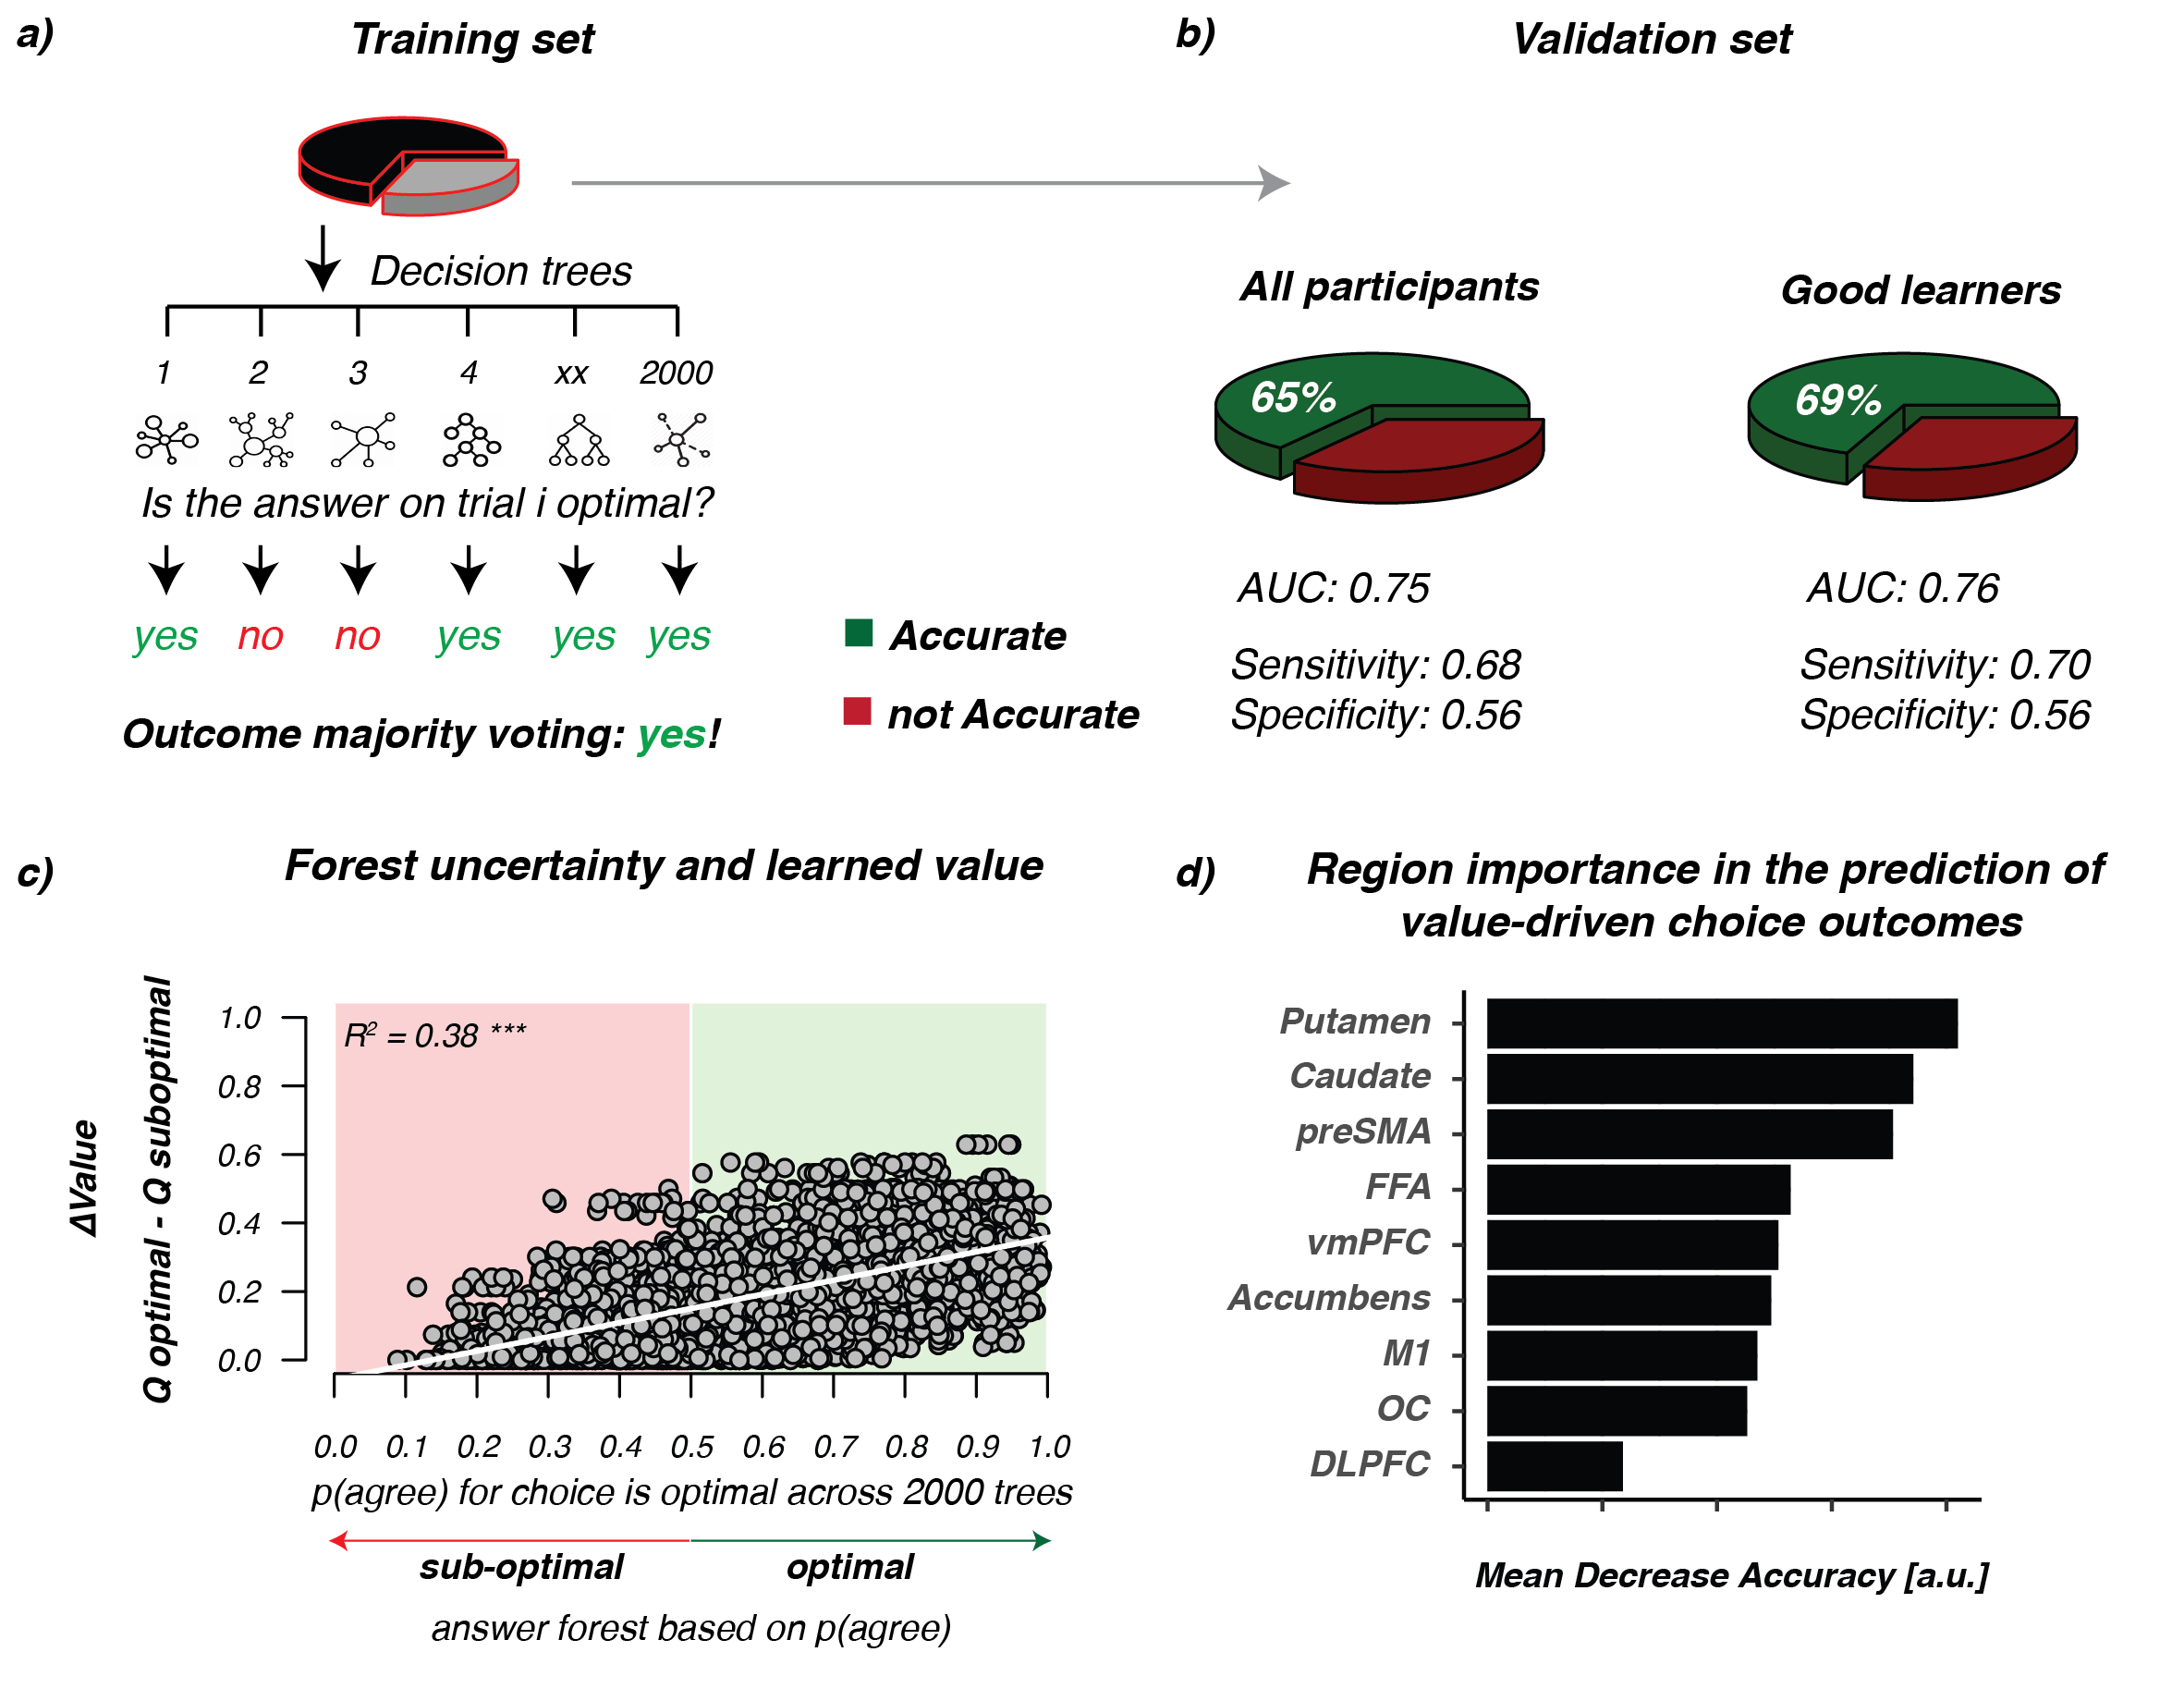
\includegraphics{_png/Figure6.png}
\caption{\textbf{Random Forest performance and importance ranking.} The
prediction of value-driven choice outcomes in the transfer phase using
trial-by-trial BOLD responses from striatal, perceptual, and prefrontal
cortex regions. (\textbf{a}) Overview of the Random Forest approach
where the training-set is used to predict choice outcomes for each trial
by using the majority vote of 2000 different decision trees. Each tree
is built using a different set, or sample, of trials and predictors from
the training set. The forest is trained on a training set sampled from
all participants (N=43), or only `the good learners' (N=34).
(\textbf{b}) Shows the classification, or decoding, accuracy (green)
given the separate unseen validation sets, for all participants and good
learners. (\textbf{c}) Plotted relationship between forest uncertainty
(i.e., proportion of agreement across 2000 trees), on each
prediction/trial (x-axis) and \(\Delta\)Value (y-axis) for the model
with the highest accuracy (i.e., the good learners). \(\Delta\)Value was
computed for each trial in the transfer phase by using the end beliefs
(\(Q\)) that participants had about each stimulus (A-to-F) at the end of
the learning phase. Forest uncertainty is defined as the proportion of
trees saying `yes! the choice on this trial was optimal'. When this
ratio is bellow 0.5 the forest will predict `no' (sub-optimal),
otherwise the prediction is `yes! the choice on this trial was optimal'
(optimal). \(R^2\)=adjusted \(R^2\). Note that, the same pattern was
found for all participants (\(R^2\)\(=0.41^{***}\), please see
supplementary Figure 3). (\textbf{d}) Plotted ranking of the ROI's in
their contribution to the predictive accuracy of the best performing
model (i.e., good learners). \label{Figure 6}}
\end{figure}

\hypertarget{discussion}{%
\section{Discussion}\label{discussion}}

This study provides novel insights into how reinforcements modulate
visual activity and specifies its potential in the prediction of future
value-driven choice outcomes. First, by focusing on how participants
learn, we find BOLD in visual regions to change with trial-by-trial
adaptations in value beliefs about the faces presented, and then to be
subsequently scaled by the signed RPE after feedback. Next, the
relevance of these observed value and feedback modulations was sought by
exploring the prediction of future value-driven choice outcomes in a
follow-up transfer phase where feedback was omitted. Our machine
learning algorithm here shows a classification accuracy of \(69\%\) for
participants who were efficient in learning by combining trial-by-trial
BOLD estimates from perceptual, striatal, and prefrontal regions. The
evaluation of region importance in these predictions ranked the FFA just
after the dorsal striatum and the preSMA, thereby showing an important
role for visual regions in the prediction of future value-driven choice
outcomes in a phase where learning is established.

In a choice between two faces, BOLD responses in both the dorsal
striatum and perceptual regions were affected more by values of the
chosen face, relative to the unchosen face. Across three levels of
uncertainty, we only observed the differential modulation of value on
BOLD when belief representations were stable. This specificity aligns
with neuronal responses to perceptual stimuli in the caudate tail (Kim
et al. 2017), visual cortex (Shuler and Bear 2006; Weil et al. 2010;
Cicmil et al. 2015), and imaging work across sensory modalities
(Serences 2008; Serences and Saproo 2010; LimOdoherty2013; Pleger et al.
2009; Kahnt et al. 2011; Vickery et al. 2011; FitzGerald et al. 2013;
Kaskan et al. 2016), where it fuels theories in which the learning of
stable reward expectations can develop to modulate, or sharpen, the
representation of sensory information critical for perceptual decision
making (Roelfsema et al. 2010; Kahnt et al. 2011; Cicmil et al. 2015).

After a choice was made, feedback modulations of signed (`valence') and
unsigned (`surprise') RPEs (Fouragnan et al. 2018) were evaluated on
BOLD responses, by using an orthogonal design where the unsigned and
signed RPE compete to explain BOLD variances. Both visual and striatal
regions respond to prediction errors (Den Ouden et al. 2012). In the
striatum both valence and surprise are thought to optimize future action
selection in the dorsal striatum, or the prediction of future rewards in
the ventral striatum. In perceptual regions, a mismatch between the
expected and received outcome is often explained as surprise where a
boost in attention or salience changes the representation of an image
without a representation of value per se. We found positive modulatory
effects of signed RPEs in all striatal regions, as well as, in the FFA
and OC. Concurrently, modulations of unsigned RPEs were only observed in
the accumbens (ventral striatum) and FFA, where notably the direction of
modulation was reversed. We speculate that this contrast arises from the
differential role of the regions. In the FFA, specialized and dedicated
information processing is essential to quickly recognize valuable face
features. Complementary boosts of surprise and valence here could
prioritize attention towards the most rewarding face feature to
strengthen the reward association in memory, or help speed up future
recognition (Gottlieb 2012; Gottlieb et al. 2014; Störmer et al. 2014).
In the accumbens, boosted effects of positive valence on BOLD were
dampened by larger mismatches. Large mismatches in what was expected are
rare in stable environments. We therefore reason that in the accumbens
the contrast between valence and surprise could function as a scale to
refine learning, eventually leading to more reliable predictions of
future rewards.

Whereas BOLD in the ventral striatum was shaped by both signed and
unsigned RPEs, the dorsal striatum was sensitive to differential value
up-to a choice and signed RPEs with the presentation of feedback (Kaskan
et al. 2016; Lak et al. 2016, 2017; McCoy et al. 2018; Van Slooten et
al. 2018). The concurrent modulation of differential value in the
primary motor cortex (please see M1 in supplementary Figure 1)
associates the dorsal striatum with the integration of sensory
information (Ding and Gold 2010; Yamamoto et al. 2012; Hikosaka et al.
2013; Kim et al. 2017), where increased visual cortex BOLD responses to
faces with the highest value could potentially help bias the outcome of
a value-driven choice.

We explored this line of reasoning with the prediction of value-driven
choice outcomes in a follow-up transfer phase after leaning. In recent
years, machine learning approaches have become increasingly important in
neuroscience (Naselaris et al. 2011; Hassabis et al. 2017; Hebart and
Baker 2018; Snoek et al. 2019), where the ease of interpretation has
often motivated a choice for linear methods above non-linear methods
(Naselaris et al. 2011; Kriegeskorte and Douglas 2018). Despite the
latter being less constrained and able to reach a better classification
accuracy by capturing non-arbitrary, or unexpected relationships (King
et al. 2018). Value-driven choices after a phase of initial learning are
influenced by the consistency of past learning, memory updating, and
attention. All of these processes are affected by both linear and
non-linear neurotransmitter modulations (Aston-Jones and Cohen 2005; Yu
and Dayan 2005; Cools and D'Esposito 2011; Beste et al. 2018). Our RF
approach was unconstrained by linearity with classification accuracies
well above chance and improved with the evaluation of only the good
learners; despite substantial decreases in data given to the algorithm
to learn the correct labelling. Critically, we additionally found that
the uncertainty of trial-by-trial predictions made by RF is tied to the
differentiability of value beliefs -- an index that we could compute for
the novel pair combination in the transfer phase by using the value
(\(Q\)) beliefs that participants had about each face at the end of
learning. These results showcase how trial-by-trial BOLD fluctuations in
striatal, prefrontal, and sensory regions can be combined by machine
learning, or decoding, algorithms to reliably predict the outcome of a
value-driven choice. Where we refine the interpretation of non-linear
predictions by combining the RF output with cognitive computational
modelling. With this combiantion we essentially show how the uncertainty
of RF predictions is tied to value beliefs acquired with learning in the
past.

An important evaluation intended with our machine learning approach was
the ranking of regions by their contribution to the predictive
(decoding) accuracy in the transfer phase. After the observed
modulations of BOLD in the learning phase this explorative analysis
sought the relevance of learning-BOLD relationships in the resolve of
future choices. Here, the ranking made by RF first identified signals
from the dorsal striatum (putamen and caudate) as most important
followed by the preSMA, and then most notably, visual regions. That is,
when the quality of leaning was high across participants, FFA ranked
just above traditional regions such as the vmPFC and the accumbens
(O'Doherty et al. 2003, 2017; Hare et al. 2011; Niv et al. 2012; Klein
et al. 2017). Notably, FFA was replaced by OC in ranking with the
evaluation of all participants (please see supplementary Figure 3b).
This difference could occur because the quality of learning was more
variable across all participants, or because RF predictions based on the
heterogeneous data from all participants were less accurate. In general,
the shift in ranking implies that when learning is less consistent
choice outcomes are better predicted by fluctuations in OC - perhaps
with the identification of rewarding low-level features. With better or
more consistent learning, however, participants should increasingly rely
on memory and specialized visual areas. Thus, search for specific face
features associated with high value by recruiting the FFA in the visual
ventral stream. Consistent with this reasoning recent neuronal
recordings show rapid visual processing of category-specific value cues
in the ventral visual stream. These specific value cues are only seen
for well-learned reward categories, and critically, precede the
processing of value in prefrontal cortex (Sasikumar et al. 2018).

We note that although BOLD fluctuations in the preSMA ranked second in
the prediction of value-driven choice outcomes, no reliable modulations
of BOLD were observed by either differential value or RPEs in the
learning phase. The preSMA is densely connected to the dorsal striatum
and consistently associated with action-reward learning (Jocham et al.
2016), or choice difficulty (Shenhav et al. 2014). The lack of
associations in this study might result from our noisier estimates of
the BOLD response that is typical for regions in the prefrontal cortex
(Pircalabelu et al. 2015; Bhandari et al. 2018), the anatomical masks
selected, or smaller variability across trials in the learning phase
(i.e., 3 pairs in learning-phase vs 15 pairs in transfer-phase).
Nevertheless, the importance indicated by RF, combined with our previous
analysis of this transfer phase data (Jahfari et al. 2018), implies an
important role for the preSMA in the resolve of value-driven choices in
concert with the striatum. More research with optimized sequences to
estimate BOLD in PFC is required to clarify the link between learning
and transfer.

To summarize, we find an important role for perceptual regions in the
prediction of future value-driven choice outcomes, which coincides with
the sensitivity of BOLD in visual regions to differential value and
signed feedback. These findings imply visual regions to learn prioritize
high value features with the integration of feedback, to support and
fasten, optimal response selection via the dorsal striatum in future
encounters.

\hypertarget{acknowledgements}{%
\section{Acknowledgements}\label{acknowledgements}}

This work was supported by an ABC Talent grant to SJ from the University
of Amsterdam, an ERC grant ERC-2012-AdG-323413 to JT, and NWO-CAS grant
012.200.012 to TK.

\hypertarget{author-contribution}{%
\section{Author contribution}\label{author-contribution}}

SJ and TK developed the questions and analysis plan for the re-analysis.
SJ and TK contributed novel methods and analyzed the data. SJ wrote the
first draft of the MS with edits from TK. JT commented on the final
draft.

\hypertarget{data-availability}{%
\section{Data availability}\label{data-availability}}

The code and preprocessed files for behavioral and decoding analyses can
be download from: \url{https://github.com/sarajahfari/Pearl3T.git}, and
fMRI preprocessing and deconvolution analysis code are available at
\url{https://github.com/tknapen/pearl_3T}. The raw data can be
downloaded from openfMRI in BIDS after acceptance of this MS.

\hypertarget{references}{%
\section*{References}\label{references}}
\addcontentsline{toc}{section}{References}

\hypertarget{refs}{}
\leavevmode\hypertarget{ref-Astonetal2005}{}%
Aston-Jones G, Cohen JD. 2005. An integrative theory of locus
coeruleus-norepinephrine function: Adaptive gain and optimal
performance. Annu Rev Neurosci. 28:403--450.

\leavevmode\hypertarget{ref-Atallahetal2007}{}%
Atallah HE, Lopez-Paniagua D, Rudy JW, O'Reilly RC. 2007. Separate
neural substrates for skill learning and performance in the ventral and
dorsal striatum. Nature neuroscience. 10:126--131.

\leavevmode\hypertarget{ref-Beckmannetal2003}{}%
Beckmann CF, Jenkinson M, Smith SM. 2003. General multilevel linear
modeling for group analysis in fmri. Neuroimage. 20:1052--1063.

\leavevmode\hypertarget{ref-Besteetal2018}{}%
Beste C, Adelhöfer N, Gohil K, Passow S, Roessner V, Li S-C. 2018.
Dopamine modulates the efficiency of sensory evidence accumulation
during perceptual decision making. International Journal of
Neuropsychopharmacology.

\leavevmode\hypertarget{ref-Bhandarietal2018}{}%
Bhandari A, Gagne C, Badre D. 2018. Just above chance: Is it harder to
decode information from human prefrontal cortex blood oxygenation
level-dependent signals? Journal of cognitive neuroscience. 1--26.

\leavevmode\hypertarget{ref-Breiman2001}{}%
Breiman L. 2001. Random forests. Machine learning. 45:5--32.

\leavevmode\hypertarget{ref-Breiman2004}{}%
Breiman L. 2004. Consistency for a simple model of random forests.

\leavevmode\hypertarget{ref-Cicmiletal2015}{}%
Cicmil N, Cumming BG, Parker AJ, Krug K. 2015. Reward modulates the
effect of visual cortical microstimulation on perceptual decisions.
Elife. 4:e07832.

\leavevmode\hypertarget{ref-CollinsFrank2014}{}%
Collins AGE, Frank MJ. 2014. Opponent actor learning (opal): Modeling
interactive effects of striatal dopamine on reinforcement learning and
choice incentive. Psychological review. 121:337--366.

\leavevmode\hypertarget{ref-CoolsDesposito2011}{}%
Cools R, D'Esposito M. 2011. Inverted-u--shaped dopamine actions on
human working memory and cognitive control. Biological psychiatry.
69:e113--e125.

\leavevmode\hypertarget{ref-Daw2011}{}%
Daw ND. 2011. Trial-by-trial data analysis using computational models.
Decision making, affect, and learning: Attention and performance XXIII.
23:3--38.

\leavevmode\hypertarget{ref-Dawetal2006}{}%
Daw ND, O'doherty JP, Dayan P, Seymour B, Dolan RJ. 2006. Cortical
substrates for exploratory decisions in humans. Nature. 441:876--879.

\leavevmode\hypertarget{ref-Denoudenetal2012}{}%
Den Ouden HEM, Kok P, De Lange FP. 2012. How prediction errors shape
perception, attention, and motivation. Frontiers in psychology. 3:548.

\leavevmode\hypertarget{ref-DingGold2010}{}%
Ding L, Gold JI. 2010. Caudate encodes multiple computations for
perceptual decisions. Journal of Neuroscience. 30:15747--15759.

\leavevmode\hypertarget{ref-Fernandezetal2001}{}%
Fernandez-Ruiz J, Wang J, Aigner TG, Mishkin M. 2001. Visual habit
formation in monkeys with neurotoxic lesions of the ventrocaudal
neostriatum. Proceedings of the National Academy of Sciences.
98:4196--4201.

\leavevmode\hypertarget{ref-Fitzgeraldetal2013}{}%
FitzGerald THB, Friston KJ, Dolan RJ. 2013. Characterising reward
outcome signals in sensory cortex. Neuroimage. 83:329--334.

\leavevmode\hypertarget{ref-Fouragnanetal2018}{}%
Fouragnan E, Retzler C, Philiastides MG. 2018. Separate neural
representations of prediction error valence and surprise: Evidence from
an fMRI meta-analysis. Human brain mapping.

\leavevmode\hypertarget{ref-Franketal2007}{}%
Frank MJ, Moustafa AA, Haughey HM, Curran T, Hutchison KE. 2007. Genetic
triple dissociation reveals multiple roles for dopamine in reinforcement
learning. Proceedings of the National Academy of Sciences.
104:16311--16316.

\leavevmode\hypertarget{ref-Gottlieb2012}{}%
Gottlieb J. 2012. Attention, learning, and the value of information.
Neuron. 76:281--295.

\leavevmode\hypertarget{ref-Gottliebetal2014}{}%
Gottlieb J, Hayhoe M, Hikosaka O, Rangel A. 2014. Attention, reward, and
information seeking. Journal of Neuroscience. 34:15497--15504.

\leavevmode\hypertarget{ref-Hareetal2011}{}%
Hare TA, Schultz W, Camerer CF, O'Doherty JP, Rangel A. 2011.
Transformation of stimulus value signals into motor commands during
simple choice. Proceedings of the National Academy of Sciences.
108:18120--18125.

\leavevmode\hypertarget{ref-Hassabisetal2017}{}%
Hassabis D, Kumaran D, Summerfield C, Botvinick M. 2017.
Neuroscience-inspired artificial intelligence. Neuron. 95:245--258.

\leavevmode\hypertarget{ref-HebartBaker2018}{}%
Hebart MN, Baker CI. 2018. Deconstructing multivariate decoding for the
study of brain function. Neuroimage. 180:4--18.

\leavevmode\hypertarget{ref-Hikosakaetal2014}{}%
Hikosaka O, Kim HF, Yasuda M, Yamamoto S. 2014. Basal ganglia circuits
for reward value--guided behavior. Annual review of neuroscience.
37:289--306.

\leavevmode\hypertarget{ref-Hikosakaetal2013}{}%
Hikosaka O, Yamamoto S, Yasuda M, Kim HF. 2013. Why skill matters.
Trends in cognitive sciences. 17:434--441.

\leavevmode\hypertarget{ref-Jahfarietal2018}{}%
Jahfari S, Ridderinkhof KR, Collins AGE, Knapen T, Waldorp LJ, Frank MJ.
2018. Cross-task contributions of frontobasal ganglia circuitry in
response inhibition and conflict-induced slowing. Cerebral Cortex.
bhy076.

\leavevmode\hypertarget{ref-JahfariTheeuwes2017}{}%
Jahfari S, Theeuwes J. 2017. Sensitivity to value-driven attention is
predicted by how we learn from value. Psychonomic bulletin \& review.
24:408--415.

\leavevmode\hypertarget{ref-Jahfarietal2015}{}%
Jahfari S, Waldorp L, Ridderinkhof KR, Scholte HS. 2015. Visual
information shapes the dynamics of corticobasal ganglia pathways during
response selection and inhibition. Journal of cognitive neuroscience.
27:1344--1359.

\leavevmode\hypertarget{ref-Jochametal2016}{}%
Jocham G, Boorman E, Behrens T. 2016. Neuroscience of value-guided
choice. The Wiley Handbook on the Cognitive Neuroscience of Learning.
554--591.

\leavevmode\hypertarget{ref-Jochametal2011}{}%
Jocham G, Klein TA, Ullsperger M. 2011. Dopamine-mediated reinforcement
learning signals in the striatum and ventromedial prefrontal cortex
underlie value-based choices. Journal of Neuroscience. 31:1606--1613.

\leavevmode\hypertarget{ref-Joeletal2002}{}%
Joel D, Niv Y, Ruppin E. 2002. Actor--critic models of the basal
ganglia: New anatomical and computational perspectives. Neural networks.
15:535--547.

\leavevmode\hypertarget{ref-Kahntetal2011}{}%
Kahnt T, Heinzle J, Park SQ, Haynes J-D. 2011. Decoding different roles
for vmPFC and dlPFC in multi-attribute decision making. Neuroimage.
56:709--715.

\leavevmode\hypertarget{ref-Kahntetal2009}{}%
Kahnt T, Park SQ, Cohen MX, Beck A, Heinz A, Wrase J. 2009. Dorsal
striatal--midbrain connectivity in humans predicts how reinforcements
are used to guide decisions. Journal of Cognitive Neuroscience.
21:1332--1345.

\leavevmode\hypertarget{ref-Kaskanetal2016}{}%
Kaskan PM, Costa VD, Eaton HP, Zemskova JA, Mitz AR, Leopold DA,
Ungerleider LG, Murray EA. 2016. Learned value shapes responses to
objects in frontal and ventral stream networks in macaque monkeys.
Cerebral Cortex. 27:2739--2757.

\leavevmode\hypertarget{ref-Kimetal2017}{}%
Kim HF, Amita H, Hikosaka O. 2017. Indirect pathway of caudal basal
ganglia for rejection of valueless visual objects. Neuron. 94:920--930.

\leavevmode\hypertarget{ref-KimHikosaka2013}{}%
Kim HF, Hikosaka O. 2013. Distinct basal ganglia circuits controlling
behaviors guided by flexible and stable values. Neuron. 79:1001--1010.

\leavevmode\hypertarget{ref-Kingetal2018}{}%
King J-R, Gwilliams L, Holdgraf C, Sassenhagen J, Barachant A, Engemann
D, Larson E, Gramfort A. 2018. Encoding and decoding neuronal dynamics:
Methodological framework to uncover the algorithms of cognition.

\leavevmode\hypertarget{ref-Kleinetal2017}{}%
Klein TA, Ullsperger M, Jocham G. 2017. Learning relative values in the
striatum induces violations of normative decision making. Nature
Communications. 8:16033.

\leavevmode\hypertarget{ref-KnapenGee2016}{}%
Knapen T, Gee J. 2016. FIRDeconvolution.

\leavevmode\hypertarget{ref-Kravitzetal2013}{}%
Kravitz DJ, Saleem KS, Baker CI, Ungerleider LG, Mishkin M. 2013. The
ventral visual pathway: An expanded neural framework for the processing
of object quality. Trends in cognitive sciences. 17:26--49.

\leavevmode\hypertarget{ref-KriegeskorteDouglas2018}{}%
Kriegeskorte N, Douglas PK. 2018. Interpreting encoding and decoding
models. arXiv preprint arXiv:181200278.

\leavevmode\hypertarget{ref-Laketal2017}{}%
Lak A, Nomoto K, Keramati M, Sakagami M, Kepecs A. 2017. Midbrain
dopamine neurons signal belief in choice accuracy during a perceptual
decision. Current Biology. 27:821--832.

\leavevmode\hypertarget{ref-Laketal2016}{}%
Lak A, Stauffer WR, Schultz W. 2016. Dopamine neurons learn relative
chosen value from probabilistic rewards. Elife. 5:e18044.

\leavevmode\hypertarget{ref-Limetal2011}{}%
Lim S-L, O'Doherty JP, Rangel A. 2011. The decision value computations
in the vmPFC and striatum use a relative value code that is guided by
visual attention. Journal of Neuroscience. 31:13214--13223.

\leavevmode\hypertarget{ref-Limetal2013}{}%
Lim S-L, O'Doherty JP, Rangel A. 2013. Stimulus value signals in
ventromedial pfc reflect the integration of attribute value signals
computed in fusiform gyrus and posterior superior temporal gyrus.
Journal of Neuroscience. 33:8729--8741.

\leavevmode\hypertarget{ref-Mccoyetal2018}{}%
McCoy B, Jahfari S, Engels G, Knapen T, Theeuwes J. 2018. Dopaminergic
medication reduces striatal sensitivity to negative outcomes in
parkinson's disease. bioRxiv.

\leavevmode\hypertarget{ref-Montagueetal1996}{}%
Montague PR, Dayan P, Sejnowski TJ. 1996. A framework for mesencephalic
dopamine systems based on predictive hebbian learning. Journal of
neuroscience. 16:1936--1947.

\leavevmode\hypertarget{ref-Naselarisetal2011}{}%
Naselaris T, Kay KN, Nishimoto S, Gallant JL. 2011. Encoding and
decoding in fMRI. Neuroimage. 56:400--410.

\leavevmode\hypertarget{ref-Nivetal2012}{}%
Niv Y, Edlund JA, Dayan P, O'Doherty JP. 2012. Neural prediction errors
reveal a risk-sensitive reinforcement-learning process in the human
brain. Journal of Neuroscience. 32:551--562.

\leavevmode\hypertarget{ref-Odohertyetal2003}{}%
O'Doherty J, Critchley H, Deichmann R, Dolan RJ. 2003. Dissociating
valence of outcome from behavioral control in human orbital and ventral
prefrontal cortices. Journal of neuroscience. 23:7931--7939.

\leavevmode\hypertarget{ref-Odohertyetal2004}{}%
O'Doherty J, Dayan P, Schultz J, Deichmann R, Friston K, Dolan RJ. 2004.
Dissociable roles of ventral and dorsal striatum in instrumental
conditioning. Science. 304:452--454.

\leavevmode\hypertarget{ref-Odohertyetal2017}{}%
O'Doherty JP, Cockburn J, Pauli WM. 2017. Learning, reward, and decision
making. Annual review of psychology. 68:73--100.

\leavevmode\hypertarget{ref-Odohertyetal2007}{}%
O'Doherty JP, Hampton A, Kim H. 2007. Model-based fMRI and its
application to reward learning and decision making. Annals of the New
York Academy of sciences. 1104:35--53.

\leavevmode\hypertarget{ref-Pircalabeluetal2015}{}%
Pircalabelu E, Claeskens G, Jahfari S, Waldorp LJ. 2015. A focused
information criterion for graphical models in fMRI connectivity with
high-dimensional data. The Annals of Applied Statistics. 9:2179--2214.

\leavevmode\hypertarget{ref-Plegeretal2009}{}%
Pleger B, Ruff CC, Blankenburg F, Klöppel S, Driver J, Dolan RJ. 2009.
Influence of dopaminergically mediated reward on somatosensory
decision-making. PLoS biology. 7:e1000164.

\leavevmode\hypertarget{ref-Roelfsemaetal2010}{}%
Roelfsema PR, Ooyen A van, Watanabe T. 2010. Perceptual learning rules
based on reinforcers and attention. Trends in cognitive sciences.
14:64--71.

\leavevmode\hypertarget{ref-Sasikumaretal2018}{}%
Sasikumar D, Emeric E, Stuphorn V, Connor CE. 2018. First-pass
processing of value cues in the ventral visual pathway. Current Biology.
28:538--548.

\leavevmode\hypertarget{ref-Schmittmannetal2015}{}%
Schmittmann VD, Jahfari S, Borsboom D, Savi AO, Waldorp LJ. 2015. Making
large-scale networks from fMRI data. PloS one. 10:e0129074.

\leavevmode\hypertarget{ref-Schultzetal1997}{}%
Schultz W, Dayan P, Montague PR. 1997. A neural substrate of prediction
and reward. Science. 275:1593--1599.

\leavevmode\hypertarget{ref-SeaboldPerktold2010}{}%
Seabold S, Perktold J. 2010. Statsmodels: Econometric and statistical
modeling with python. In: Proceedings of the 9th python in science
conference. p. 57--61.

\leavevmode\hypertarget{ref-Serences2008}{}%
Serences JT. 2008. Value-based modulations in human visual cortex.
Neuron. 60:1169--1181.

\leavevmode\hypertarget{ref-SerencesSapro2010}{}%
Serences JT, Saproo S. 2010. Population response profiles in early
visual cortex are biased in favor of more valuable stimuli. Journal of
neurophysiology. 104:76--87.

\leavevmode\hypertarget{ref-Shenhavetal2014}{}%
Shenhav A, Straccia MA, Cohen JD, Botvinick MM. 2014. Anterior cingulate
engagement in a foraging context reflects choice difficulty, not
foraging value. Nature neuroscience. 17:1249.

\leavevmode\hypertarget{ref-Shuleretal2006}{}%
Shuler MG, Bear MF. 2006. Reward timing in the primary visual cortex.
Science. 311:1606--1609.

\leavevmode\hypertarget{ref-Snoeketal2019}{}%
Snoek L, Miletić S, Scholte HS. 2019. How to control for confounds in
decoding analyses of neuroimaging data. NeuroImage. 184:741--760.

\leavevmode\hypertarget{ref-Stormer2014}{}%
Störmer V, Eppinger B, Li S-C. 2014. Reward speeds up and increases
consistency of visual selective attention: A lifespan comparison.
Cognitive, Affective, \& Behavioral Neuroscience. 14:659--671.

\leavevmode\hypertarget{ref-Tobleretal2005}{}%
Tobler PN, Fiorillo CD, Schultz W. 2005. Adaptive coding of reward value
by dopamine neurons. Science. 307:1642--1645.

\leavevmode\hypertarget{ref-vanSlootenetal2018}{}%
Van Slooten JC, Jahfari S, Knapen T, Theeuwes J. 2018. How pupil
responses track value-based decision-making during and after
reinforcement learning. PLoS computational biology. 14:e1006632.

\leavevmode\hypertarget{ref-Vickeryetal2011}{}%
Vickery TJ, Chun MM, D L. 2011. Ubiquity and specificity of
reinforcement signals throughout the human brain. Neuron". 72:166--177.

\leavevmode\hypertarget{ref-WatkinsDayan1992}{}%
Watkins CJCH, Dayan P. 1992. Q-learning. Machine learning. 8:279--292.

\leavevmode\hypertarget{ref-Weiletal2010}{}%
Weil RS, Furl N, Ruff CC, Symmonds M, Flandin G, Dolan RJ, Driver J,
Rees G. 2010. Rewarding feedback after correct visual discriminations
has both general and specific influences on visual cortex. American
Journal of Physiology-Heart and Circulatory Physiology. 104:1746--1757.

\leavevmode\hypertarget{ref-Woolrichetal2001}{}%
Woolrich MW, Ripley BD, Brady M, Smith SM. 2001. Temporal
autocorrelation in univariate linear modeling of fMRI data. Neuroimage.
14:1370--1386.

\leavevmode\hypertarget{ref-Yamamotoetal2012}{}%
Yamamoto S, Monosov IE, Yasuda M, Hikosaka O. 2012. What and where
information in the caudate tail guides saccades to visual objects.
Journal of Neuroscience. 32:11005--11016.

\leavevmode\hypertarget{ref-YuDayan2005}{}%
Yu AJ, Dayan P. 2005. Uncertainty, neuromodulation, and attention.
Neuron. 46:681--692.


\end{document}
